\documentclass[a4paper,10pt]{book} %type de document et paramètres


\usepackage[utf8]{inputenc} %package fondamental
\usepackage[T1]{fontenc} %package fondamental
\usepackage[english,francais]{babel} %package de langues
\usepackage{lmodern} %police de caractère

\usepackage[top=3cm, bottom=3cm, left=4cm, right=2cm]{geometry} %permet de paramétrer les marges par défaut
\usepackage{changepage} %permet de modifier localement une mise en page (marges,...) : utilisé pour la page de garde
\usepackage{multicol} %permet de mettre plusieurs colonnes (\begin{multicols}{2} \end{multicols} jusqu'à 10 colonnes)
\usepackage[pdftex, pdfauthor={Pierre Gimalac}, pdftitle={Analyse Élémentaire II}, pdfsubject={Mathématiques, Analyse}, pdfkeywords={Mathématiques, Analyse}, colorlinks=true, linkcolor=black]{hyperref} %permet de se déplacer dans le pdf depuis le sommaire en cliquant sur les titres, ainsi que de parametrer les meta données du PDF
\usepackage{url} %permet de mettre des URL actifs \url{}
\let\urlorig\url
\renewcommand{\url}[1]{\begin{otherlanguage}{english}\urlorig{#1}\end{otherlanguage}}

\usepackage{mathtools,amssymb,amsthm} %maths
\usepackage{mathrsfs} %maths (par exemple les lettres caligraphiées)
\usepackage{stmaryrd} %maths (par exemple les ensembles d'entiers)
\usepackage{calrsfs} %maths (par exemple les notations des ensembles)
\usepackage{yhmath} % permet de noter les arcs de cercle avec \wideparen{AOB}
%\usepackage{xlop} %permet d'afficher des opérations mathématiques
\usepackage[squaren,Gray]{SIunits} %permet de noter des unités proprement

\usepackage{graphicx} %permet d'insérer des images proprement (ajoute des parametres)
\usepackage{setspace} %permet de modifier localement l'interligne
\usepackage{wrapfig} %permet de mettre des images à coté d'un texte
\usepackage{enumitem} %permet de personnaliser les listes
\usepackage{pdfpages} %permet d'insérer un pdf \includepdf[pages={1-2}]{truc.pdf}

\usepackage{tikz} %package trop bien permet de dessiner tout et n'importe quoi ! \begin{tikzpicture}
%\usepackage{circuitikz} %permet de dessiner des circuits logiques (entre autre) avec la syntaxe de tikz (\begin{circuitikz}) par exemple \node[american not port] pour le 'non'


\newcommand{\R}{\mathbb{R}}
\newcommand{\Rpe}{\mathbb{R}_{+}^{*}}
\newcommand{\N}{\mathbb{N}}
\newcommand{\Z}{\mathbb{Z}}
\newcommand{\C}{\mathbb{C}}
\newcommand{\Q}{\mathbb{Q}}
\newcommand{\K}{\mathbb{K}}
\newcommand{\tvi}{théorème des valeurs intermédiaires}
\newcommand{\taf}{théorème des accroissements finis}
\newcommand{\edl}{équation différentielle linéaire }
\newcommand{\edlh}{\edl homogène }


\begin{document}

\begin{titlepage}
\newgeometry{margin=2.7cm}
\thispagestyle{empty}
\begin{center}
\vspace*{7cm}
\Huge \textsc{Analyse Élémentaire II}\\
\vspace{1.5cm}
\Large Pierre Gimalac\\
\vspace{0.5cm}
\large \textit{Licence de Mathématiques}
\vfill
\end{center}
\large \textit{Janvier - Mai 2017}
\hfill 
\large Cours de Kevin Carrier
\restoregeometry
\end{titlepage}

\renewcommand{\contentsname}{Sommaire}
\thispagestyle{empty}
\tableofcontents
\thispagestyle{empty}
\chapter{Fonctions continues}
\section{Limite de fonctions}
\subsection{Définition}
Soient $f$ une fonction de $E=[a;b]$ dans $F=\R$ avec a et b $\in \R\cup\{\infty\}$et c un réel de $]a;b[$.

\subsubsection{Limite finie en un réel}
$\lim\limits_{x\rightarrow c} f(x)=l \Leftrightarrow \forall \epsilon >0$, $\exists \eta>0$ tel que $\forall x\in E\backslash\{c\}$, $|x-c|<\eta \Rightarrow |f(x)-l|\leq \epsilon$\\\\

\textit{Limite à gauche :}\\
$\lim\limits_{\substack{x\rightarrow c \\ x<c}} f(x)=l \Leftrightarrow \forall \epsilon>0$, $\exists \eta>0$ tel que $\forall x\in E\backslash\{c\}$, $c-\eta\leq x<c \Rightarrow |f(x)-l|<\epsilon$\\

\textit{Limite à droite :}\\
$\lim\limits_{\substack{x\rightarrow c \\ x>c}} f(x)=l \Leftrightarrow \forall \epsilon>0$, $\exists \eta>0$ tel que $\forall x\in E\backslash\{c\}$, $c<x\leq c+\eta \Rightarrow |f(x)-l|<\epsilon$\\

\subsubsection{Limite finie en l'infini}
$\lim\limits_{x\rightarrow \infty} f(x)=l \Leftrightarrow \forall \epsilon>0$, $\exists M>a$ tel que $\forall x\geq M$, $|f(x)-l|<\epsilon$

\subsubsection{Limite infinie en un réel}
$\lim\limits_{x\rightarrow c}f(x)=+\infty \Leftrightarrow \forall N>0$, $\exists \eta>0$ tel que $\forall x\in ]a;b[$, $|x-c|<\eta \Rightarrow f(x)>N$\\\\

\textit{Limite à gauche :}\\
$\lim\limits_{\substack{x\rightarrow c \\ x<c}}f(x)=+\infty \Leftrightarrow \forall N>0, \exists \eta>0$ tel que $\forall x\in ]a;c[$, $c-x<\eta \Rightarrow f(x)>N$\\

\textit{Limite à droite :}\\
$\lim\limits_{\substack{x\rightarrow c \\ x>c}} f(x)=+\infty \Leftrightarrow \forall N>0$, $\exists \eta>0$ tel que $\forall x\in ]a;c[$, $x-c<\eta \Rightarrow f(x)>N$

\subsubsection{Limite infinie en l'infini}
$\lim\limits_{x\rightarrow +\infty} f(x)=+\infty \Leftrightarrow \forall N>0$, $\exists M>a$ tel que $\forall x >M$, $f(x)>N$

\newpage

\subsection{Unicité de la limite}
\subsubsection{Théorème}
La limite d'une fonction est unique.

\subsubsection{Preuve}
On va démontrer ce théorème en supposant qu'il existe $l_{1}$ et $l_{2}$ vérifiant la définition,\begin{enumerate}
\item $\forall \epsilon_{1}>0$, $\exists \eta_{1}>0$ tel que $\forall x\in ]a;b[$, $|x-c|<\eta_{1} \Rightarrow |f(x)-l_{1}| <\epsilon_{1}$
\item $\forall \epsilon_{2}>0$, $\exists \eta_{2}>0$ tel que $\forall x\in ]a;b[$, $|x-c|<\eta_{2} \Rightarrow |f(x)-l_{2}| <\epsilon_{2}$\\ \end{enumerate}

On a $|x-c|<min(\eta_{1},\eta_{2})$.\\

Si l'on prend $\epsilon_{1}=\epsilon_{2}=\frac{\epsilon}{2}$, on obtient $|l_{1}-l_{2}|=|l_{1}-f(x)+f(x)-l_{2}|$\\
\hspace*{7,4cm} $\leq |l_{1}-f(x)| + |l_{2}-f(x)|$ \\
\hspace*{7,4cm} $\leq \frac{\epsilon}{2}+\frac{\epsilon}{2}=\epsilon$\\

Ainsi en faisant tendre $\epsilon$ vers 0, $l_{1}=l_{2}$.

\subsection{Existence d'une limite}
La limite d'une fonction en un point existe si et seulement si les limites à gauche et à droite en ce point existent et sont égales.

\subsection{Caractérisation séquentielle de la limite}
\emph{Théorème}\\
Soient $f : $I$ \rightarrow \R$, $c\in I$ et $l\in \R\cup\{+\infty\}$. $\lim\limits_{x\rightarrow c} f(x)=l$ est équivalent à $\lim\limits_{n\rightarrow +\infty} f(U_{n})=l$ pour toute suite $(U_{n})_{n\geq 0}$ telle que $\forall n \geq 0$, $U_{n} \in I$,  $U_{n}\neq c$ et $\lim\limits_{n\rightarrow +\infty} U_{n}=c$.

\subsection{Opérations sur les limites}
Soient $f, $g$ : $I$ \rightarrow \R$ telles que $\lim\limits_{x\rightarrow c} f(x)=l$ et $\lim\limits_{x\rightarrow c} g(x)=m$
(avec m et l finies ou infinies et $c \in \overline{I}=[a;b]$ et avec a et b finis ou infinis). Si les opérations sont valides, on a:
\begin{enumerate}
\item\textbf{Valeur absolue}\\
$\lim\limits_{x\rightarrow c}|f(x)|=|l|$\\

\item \textbf{Somme}\\
$\lim\limits_{x\rightarrow c} [f(x)+g(x)]=l+m$\\

\item\textbf{Produit}\\
$\lim\limits_{x\rightarrow c} [f(x)g(x)]=l\times m$\\

\item\textbf{Multiplication par un scalaire}\\
$\lim\limits_{x\rightarrow c} \lambda f(x)=\lambda l$ avec $\lambda\in \R$\\

\item\textbf{Quotient}\\
Si $l\neq 0$, $\lim\limits_{x\rightarrow c} \frac{g(x)}{f(x)}=\frac{m}{l}$.\\

\item\textbf{Composition de fonctions}\\
Si $\lim\limits_{y\rightarrow l}g(y)=g(l)$, $\lim\limits_{x\rightarrow c}g\circ f(x)=\lim\limits_{y \rightarrow l}g(y)$.
\end{enumerate}

\subsubsection{Démonstrations}
\begin{enumerate}
\item \emph{Valeur absolue}\\

$\lim\limits_{x\rightarrow c}f(x)=l$ donc $\forall \epsilon>0$, $\exists \delta>0$ tel que $\forall x\in I$, $0<|{x-c}|<\delta \Rightarrow |f(x)-l|<\epsilon$.\\\\

On veut montrer que, $\forall a,b \in \R^{2}$, $|a-b|>||a|-|b||$ :\\

Si a et b sont positifs, $||a|-|b||=|a-b|$, s'ils sont négatifs $||a|-|b||=|-a+b|=|a-b|$.\\
Si $a>0$ et $b<0$, $|a-b|=a+|b|\geq |a-b|$ (inégalité triangulaire).\\
Si $a<0$ et $b>0$, $|a-b|=|b-a|=b+|a|\geq |a-b|$ (inégalité triangulaire).\\

On a donc $\forall \epsilon>0$, $\exists \delta>0$ tel que $\forall x\in I$, $0<|x-c|<\delta \Rightarrow ||f(x)|-|l||\leq|f(x)-l|<\epsilon$\\
et donc $\lim\limits_{x\rightarrow c}|f(x)|=|l|$.\\

\item \emph{Somme}\\

Soit $\epsilon>0$, on cherche un nombre positif $\delta$ tel que, pour tout x $\in$ I,\\$0<|x-c|<\delta\Rightarrow |f(x)+g(x)-(l+m)|<\epsilon$.\\

Avec l'inégalité triangulaire, on a : $|f(x)+g(x)-(l+m)|=|(f(x)-l)+(g(x)-m)|\\
\hspace*{8.95cm}\leq |(f(x)-l)|+|(g(x)-m)|$.\\

Puisque $\lim\limits_{x\rightarrow c} f(x)=l$, $\exists\delta_{1}$ tel que $\forall x$, $0<|x-c|<\delta_{1} \Rightarrow|f(x)-l|<\frac{\epsilon}{2}$.

De même, puisque $\lim\limits_{x\rightarrow c} g(x)=m$, $\exists\delta_{2}$ tel que $\forall x$, $0<|x-c|<\delta_{2} \Rightarrow|g(x)-m|<\frac{\epsilon}{2}$.\\

On a $0<|x-c|<min(\delta_{1};\delta_{2})$ d'où $\left\{\begin{array}{rcl}
|f(x)-l|&<&\frac{\epsilon}{2}\\
|g(x)-m|&<&\frac{\epsilon}{2}
\end{array} \right.$

\bigskip

On a donc $|f(x)+g(x)-(l+m)|\leq|(f(x)-l)|+|(g(x)-m)|<\epsilon$ et donc $\lim\limits_{x\rightarrow c}(f+g)(x)=l+m$.\\

\item \emph{Produit}\\

On veut montrer que $\forall \epsilon>0$, $\exists \delta$ tel que $\forall x\in I$, $0<|x-c|<\delta \Rightarrow |f(x)g(x)-lm|<\epsilon$.\\

f(x)g(x)-lm=l(g(x)-m)+m(f(x)-l)+(f(x)-l)(g(x)-m)\\

Puisque $\lim\limits_{x\rightarrow c} f(x)=l$ et $\lim\limits_{x\rightarrow c} g(x)=m$, alors $\exists\delta_{1},\delta_{2},\delta_{3},\delta_{4}>0$ tel que\\
$\forall x\in I$, $\left\{\begin{array}{rcl}
0<|x-c|<\delta_{1}&\Rightarrow &|f(x)-l|<\sqrt{\frac{\epsilon}{3}} \\
0<|x-c|<\delta_{2}&\Rightarrow &|g(x)-m|<\sqrt{\frac{\epsilon}{3}} \\
0<|x-c|<\delta_{3}&\Rightarrow &|f(x)-l|<\frac{\epsilon}{3(1+|m|)} \\
0<|x-c|<\delta_{4}&\Rightarrow &|g(x)-m|<\frac{\epsilon}{3(1+|l|)}
\end{array} \right.$

\bigskip

Soit $\delta=min(\delta_{i})$, alors $0<|x-c|<\delta \Rightarrow \left\{\begin{array}{rcl}
|f(x)-l|&<&\sqrt{\frac{\epsilon}{3}} \\
|g(x)-m|&<&\sqrt{\frac{\epsilon}{3}} \\
|f(x)-l|&<&\frac{\epsilon}{3(1+|m|)} \\
|g(x)-m|&<&\frac{\epsilon}{3(1+|l|)}
\end{array} \right.$

\bigskip

$|f(x)g(x)-lm|\leq |l||g(x)-m|+|m||f(x)-l|+|f(x)-l||g(x)-m|$\\
\hspace*{2.5cm}$\leq (1+|l|)|g(x)-m|+(1+|m|)|f(x)-l|+|f(x)-l||g(x)-m|$\\
\hspace*{2.5cm}$\leq \frac{\epsilon}{3}+\frac{\epsilon}{3}+\sqrt{\frac{\epsilon}{3}}\sqrt{\frac{\epsilon}{3}}=\epsilon$

et donc $f(x)g(x)$ tend vers $lm$.

\newpage

\item \emph{Multiplication par un scalaire}\\

On utilise la démonstration de la limite d'un produit de fonctions en posant $\lambda=h(x)$ et donc $\lim\limits_{x\rightarrow c} h(x)=\lambda$, d'où $\lim\limits_{x\rightarrow c}\lambda f(x)=\lambda l$.\\\\

\item \emph{Quotient}\\

On va montrer que $\lim\limits_{x\rightarrow c} \frac{1}{g(x)}=\frac{1}{m}$ avant d'utiliser la limite du produit ($\frac{f(x)}{g(x)}=f(x)\times \frac{1}{g(x)}$).\\

On veut donc montrer qu'il existe, pour tout $\epsilon>0$, $\delta>0$ tel que \\
$\forall x\in I$, $0<|x-c|<\delta \Rightarrow |\frac{1}{g(x)}-\frac{1}{m}|<\epsilon$.\\

On sait que $\lim\limits_{x\rightarrow c}g(x)=m$ donc que $\exists\delta_{1}$ tel que $0<|x-c|<\delta_{1}\Rightarrow |g(x)-m|<|\frac{m}{2}|$.\\

On a de plus $||g(x)|-|m||\leq|g(x)-m|$ d'où $||g(x)|-|m||<|\frac{m}{2}|$\\
\hspace*{6.5cm}$-|\frac{m}{2}|<|g(x)|-|m|<|\frac{m}{2}|$\\
\hspace*{7cm}$|\frac{m}{2}|<|g(x)|<|\frac{3m}{2}|$\\
\hspace*{7cm}$|m|<2|g(x)|<|3m|$\\
\hspace*{7cm}$\frac{1}{|g(x)|}< \frac{2}{|m|}<\frac{3}{|g(x)|}$\\

$|\frac{1}{g(x)}-\frac{1}{m}|=|\frac{m-g(x)}{mg(x)}| \leq \frac{1}{|m|}\times \frac{1}{g(x)}|\times|m-g(x)|$\\
\hspace*{1.55cm} $<\frac{1}{|m|}\times \frac{2}{|m|}\times |m-g(x)|$\\

Puisque $\frac{\epsilon}{2}|m|^{2}>0$, $\exists\delta_{2}$ tel que $\forall x\in I$, $0<|x-c|<\delta_{2}\Rightarrow |m-g(x)|<\frac{\epsilon}{2}|m|^{2}$.\\

On pose $\delta=min(\delta_{1};\delta_{2})$ et alors $\forall x\in I$, $0<|x-c|<\delta\Rightarrow |\frac{1}{g(x)}-\frac{1}{m}|<\epsilon$.\\

On a donc $\lim\limits_{x\rightarrow c}\frac{1}{g(x)}=\frac{1}{m}$ et par produit $\lim\limits_{x\rightarrow c}\frac{f(x)}{g(x)}=\frac{l}{m}$.\\\\
\end{enumerate}

\subsubsection{Limites indéterminées}
Les opérations suivantes sur des limites sont indéterminées : $0\times\infty$ ; $\frac{\infty}{\infty}$ ; $\frac{0}{0}$ ; $\infty-\infty$.\\\\

\subsection{Inégalité}
Soient $f,g : $I$ \rightarrow \R$ telles que $\lim\limits_{x\rightarrow c}f(x)=l$ et $\lim\limits_{x\rightarrow c} g(x)=m$.\\
Si $\forall x\in I$, on a $f(x)\leq g(x)$ alors $l\leq m$.

\subsubsection{Remarque}
Si $\forall x\in I$, $f(x)< g(x)$, on n'a pas nécessairement $l<m$ (on peut avoir l=m).

\newpage

\subsection{Limite et extremum}
\subsubsection{Énoncé}
Soient $f : I\subset \R\rightarrow \R$ une fonction croissante et $b=$sup$(I)$ si $I$ est majoré et $b=\infty$ sinon.\\
Si $f$ est majorée sur I, $\lim\limits_{x\rightarrow b} f(x)=$sup$ f(x)_{x\in I}$ et sinon $\lim\limits_{x\rightarrow b} f(x)=\infty$.

\subsubsection{Preuve}
Soit $(U_{n})$ une suite telle que $\forall n\in \N$, $U_{n}\in I$ et $\lim\limits_{n\rightarrow \infty} U_{n}=b$.\\

Montrons que $\lim\limits_{n\rightarrow \infty} f(U_{n})=\left\{\begin{array}{lcl}
sup(f(x))\text{ si $f$ est majorée sur $I$ }&&\\
\infty\text{ sinon }&&\end{array}\right.$

\bigskip\bigskip 

Si $f$ est majorée sur $D_{f}=$I alors on note $M=\underset{x\in D_{f}}{sup} f(x)$ le plus petit majorant de J=f(I).\\

Soit $(U_{n})_{n\geq 0}$ une suite convergeant vers b un réel, montrons que $\lim\limits_{n\rightarrow +\infty}f(U_{n})=M$.\\\\
Soit $\forall k\in \N^{*}$, $\epsilon_{k}=\frac{1}{k}$ ; $\exists N_{k}>0$ tel que $\forall n>N_{k}$, $|U_{n}-b|\leq \epsilon_{k}$.\\\\
Par définition de b et de $(U_{n})_{n\geq 0}$, on a $\forall n\geq 0$, $U_{n}\leq b$ donc $\forall \epsilon_{k}>0$, $\exists N_{k}>0$ tel que $\forall n>N_{k}$, $0\leq b-U_{n}\leq \epsilon_{k}$, c'est-à-dire $b\geq U_{n} \geq b-\epsilon_{k}$.\\

Soit $(v_{n})_{n\geq 0}$ une suite telle que $\left\{ \begin{array}{rcl}
\forall n \in \llbracket N_{k}, N_{k+1}\llbracket&\text{, }& v_{n}=b-\epsilon_{k} \\
\forall n\in \llbracket 0;N_{1}\llbracket&\text{, }& v_{n}=min(U_{n})_{0\leq n\leq N_{1}} \end{array} \right.$ \bigskip

Par construction, $(v_{n})_{n\geq 0}$ vérifie :

\begin{enumerate} \item $\left \{ \begin{array}{rcl} v_{n}\text{ croissante} \\
\text{f croissante} \end{array} \right. \Rightarrow f(v_{n})$ croissante\\
\item $\left\{ \begin{array}{rcl} \forall n\geq 0\text{, }v_{n}\leq u_{n} \\
\text{f croissante} \end{array} \right. \Rightarrow \forall n\geq 0\text{, }f(v_{n}) \leq f(U_{n})$\\
\item $\left\{\begin{array}{rcl} (v_{n})\text{ croissante} \\
f(v_{n})\text{ bornée } \end{array} \right. \Rightarrow \lim\limits_{n\rightarrow +\infty} f(v_{n})=M=\underset{x\in D_{f}}{sup} (f(x))$ \end{enumerate}

\subsection{Composition de fonctions}
Soient $f: D_{f}\rightarrow D_{g}\subset\R$ et $g:D_{f}\rightarrow \R$ et $x_{0}\in \overline{D}_{f}$.\\

On suppose que $f$ admet une limite en $x_{0}$ et on note $\lim\limits_{x\rightarrow x_{0}}f(x)=l$ alors $l\in \overline{D}_{g}$.\\

De plus, si $\lim\limits_{y\rightarrow l} g(y)$ existe alors $\lim\limits_{x\rightarrow x_{0}} (g\circ f)(x)=\lim\limits_{y\rightarrow l} g(y)$.

\subsubsection{Remarque}
Il se peut que $\lim\limits_{x\rightarrow x_{0}} (g\circ f)(x)$ existe mais pas $\lim\limits_{y\rightarrow l} g(y)$.\\

\emph{Exemple :} si $f$ est la fonction nulle alors $g(f(x))=g(0)$ et donc admet une limite en tout point. Or la limite de $g$ en 0 peut ne pas exister (par exemple si $g$ est la fonction partie entière).

\subsubsection{Preuve}
Supposons que $\lim\limits_{y\rightarrow l} g(y)$ existe et vaut l'.\\
$\forall\epsilon>0$, $\exists\eta>0$ tel que $\forall y\in D_{g}\backslash\{l\}$, $|y-l|\leq \eta \Rightarrow | g(y)-l'|\leq \epsilon$.\\

D'autre part comme $\lim\limits_{x\rightarrow x_{0}} f(x)=l$, $\exists \mu>0$ tel que $\forall x\in D_{f}\backslash\{x_{0}\}$, $|x-x_{0}|\leq \mu \Rightarrow |f(x)-l|\leq \eta$.\\
Ainsi on trouve $\exists \mu>0$ tel que $\forall x\in D_{f}\backslash\{x_{0}\}$, $|x-x_{0}|\leq \mu \Rightarrow |f(x)-l|\leq \eta \Rightarrow |g(f(x))-l'|\leq \epsilon$.

\newpage

\section{Fonctions réelles continues}
\subsection{Définition}
Soit $f : I=D_{f}\subset\R\rightarrow \R$ et $c\in I$.\\ \begin{enumerate}

\item $f$ est continue à droite en c si et seulement si $\lim\limits_{\substack{ x\rightarrow c \\ x<c}} f(x)=f(c)$.

\item Idem pour la continuité à gauche.\\

\item $f$ est continue en c si et seulement si $\lim\limits_{x\rightarrow c} f(x)=f(c)$.\\

\item $f$ est continue sur $I$ si et seulement si elle est continue en tout point de I. \end{enumerate}

\subsubsection{Remarque}
f est continue en c si et seulement si $f$ est continue à gauche et à droite.

\subsection{Démonstration de la continuité}
Pour vérifier la continuité d'une fonction en un point, il faut vérifier \begin{enumerate}
\item que $f$ est définie en c.
\item que la limite de f(x) quand x tend vers c existe.
\item que $\lim\limits_{x\rightarrow c} f(x)=f(c)$. \end{enumerate}

\subsection{Caractérisation de Weierstrass}
\emph{Théorème}\\

Soit $f$ : $D_{f}\subset \R \rightarrow \R$ et $c \in D_{f}$.\\
f est continue en c si et seulement si $\forall \epsilon>0$, $\exists \eta>0$ tel que $\forall x\in D_{f}$
$|x-c| \leq \eta \Rightarrow |f(x)-f(c)|\leq \epsilon$.

\subsubsection{Remarque} \begin{enumerate}
\item $\eta$ dépend de $\epsilon$ et $c$, on le note parfois $\eta(\epsilon,c)$ ou $\eta_{\epsilon,c}$.
\item $f$ est discontinue en c si et seulement si $\exists \epsilon>0$ tel que $\forall \eta>0$, $\exists x\in D_{f}$ tel que $|x-c|\leq \eta$ et $|f(x)-f(c)|>\epsilon$. \end{enumerate}

\subsubsection{Exemples}
\begin{enumerate}
\item fonction identité\\

\item fonctions constantes\\

\item fonctions lipschitziennes

$f:I\rightarrow \R$ est lipschitzienne s'il existe $\lambda>1$ tel que $\forall(x;y)\in I^{2}$ on ait $|f(x)-f(y)|\leq\lambda|x-y|$.\\
On peut prendre $\eta=\frac{\epsilon}{\lambda}$ pour démontrer la continuité. \end{enumerate}

\subsection{Hors programme - Continuité uniforme}
Soit $f : $I$ \rightarrow \R$, $f$ est uniformément continue sur $I$ $\Leftrightarrow \forall \epsilon>0$, $\exists \eta>0$, $\forall (x,y)\in I^{2}$,\\
$|x-y|<\eta \Rightarrow |f(x)-f(y)|<\epsilon$ ($\eta$ ne dépend pas de y contrairement à la continuité simple).

\subsection{Caractérisation avec des suites}
\subsubsection{Théorème}
Soient $f : D_{f}\subset\R \rightarrow \R$ et $c\in D_{f}$.\\
f est continue en c si et seulement si $\forall (U_{n})_{n\geq 0}\subset D_{f}$ telle que $\lim\limits_{n\rightarrow \infty}U_{n}=c$ on a $\lim\limits_{n\rightarrow \infty} f(U_{n})=f(c)$.

\subsubsection{Démonstration}
\begin{itemize}\renewcommand{\labelitemi}{$\bullet$} \item $\Rightarrow$\\
f est continue en c signifie que $\forall \epsilon>0$, $\exists \eta>0$ tel que $\forall x\in D_{f}$, $|x-c|\leq \eta \Rightarrow |f(x)-f(c)|\leq \epsilon$.\\
Posons $(U_{n})_{n\in\N}\subset D_{f}$ qui converge vers c et montrons que $f(U_{n})$ converge vers f(c) :\\

Soient $\epsilon>0$ et $\eta_{\epsilon}>0$ donné par la définition de la continuité de $f$ en c.\\
$(U_{n})$ converge vers c signifie que $\exists N\in \N$ tel que $\forall n\geq N$, on a $|U_{n}-c|\leq \eta_{\epsilon}$,\\
or par définition de la continuité de $f$ en c on a $|U_{n}-c|\leq \eta_{\epsilon} \Rightarrow |f(U_{n})-f(c)|\leq \epsilon$.\\

D'où finalement, $\forall \epsilon>0$, $\exists N\in \N$ tel que $\forall n\geq N$, on a $|f(U_{n})-c|\leq \epsilon$
et donc\\
$f(U_{n})$ converge bien vers $f(c)$.\\

\item $\Leftarrow$\\
Supposons $f$ n'est pas continue en $c$ alors $\exists\epsilon>0$ tel que $\forall\eta>0$, $\exists x_{\eta}\in D_{f}$\\
vérifiant $|x_{\eta}-c|\leq \eta$ et $|F(x_{\eta})-f(c)|>\epsilon$.\\

On construit $(U_{n})_{n\in\N}$ comme suit : $\forall n\in \N^{*}$, $U_{n}=x_{\frac{1}{n}}$\\
par construction $U_{n}$ converge vers c or $\forall n\in \N^{*}$, $|f(U_{n})-f(c)|>\epsilon$.
\end{itemize}

\subsubsection{Applications}
\begin{enumerate} \item Soit $f(x)=\left\{\begin{array}{rcl}
\frac{1}{x} & si& x\neq 0\\
0 & si& x=0
\end{array} \right.$\\
On montre que $f$ est discontinue en 0 en prenant $U_{n}=\frac{1}{n}$.\\

\item Soit $f(x)=[x]$. On montre que $f$ est discontinue en tout $z\in\Z$ en prenant $U_{n}=z-\frac{1}{n}$.\\

\item fonction de Dirichlet
$\text{Dir}(x)=\left\{\begin{array}{rcl}
1 & si& x\in\Q\\
0 & si& x\notin \Q
\end{array}\right.$ \end{enumerate}

On montre que cette fonction est discontinue en tout point de $\R$ :\\
Soit $c\in \R$, $\exists (U_{n})_{n\in \N}\subset\Q$ telle que $\lim\limits_{n\rightarrow \infty}U_{n}=c$, on prend la suite des troncatures décimales de c.\\
De plus, $(U_{n})_{n\in\N}\subset \Q$ donc $Dir(U_{n})$ converge vers 1.\\

D'autre part, soit $(v_{n})_{n\in \N^{*}}\subset \R\backslash \Q$ telle que $\forall n\in \N^{*}$, $v_{n}=U_{n}+\frac{\sqrt{2}}{n}$.\\
$v_{n}$ converge vers c et $Dir(v_{n})$ converge vers 0 car $\forall n\in \N^{*}$, $v_{n}\in \R\backslash\Q$.\\

Ainsi $U_{n}$ et $v_{n}$ convergent vers une même limite c mais $Dir(U_{n})$ et $Dir(v_{n})$ n'ont pas la même limite donc $Dir$ ne peut pas être continue.

\subsection{Continuité sur un intervalle}
On peut résumer la propriété de continuité sur un intervalle fermé borné $[a;b]$ :\\
$\forall (U_{n})_{n\in\N} \subset [a,b]$ convergente, on a $f(\lim U_{n})=\lim f(U_{n})$.

\newpage

\section{Prolongement par continuité}
\subsubsection{Énoncé}
Soit $f:D_{f}\subset \R$ et $a\notin D_{f}$.\\
Supposons que $f$ a une limite finie l au point a. On pose alors $\overset{~}{f}: \begin{array}{rcl} D_{f}\cup \{a\}&\rightarrow& \R \\
x&\mapsto &\left\{ \begin{array}{rcl}
f(x)&\text{ si }& x\in D_{f}\\
l&\text{ si }& x=a
\end{array} \right. \end{array}$

$\overset{~}{f}$ est continue au point $a$, on dira que $\overset{~}{f}$ est le prolongement par continuité de $f$ au point $a$.

\subsubsection{Remarque}
On peut ainsi ajouter des points au domaine de définition d'une fonction et conserver sa continuité.

\section{Opérations sur les fonctions continues}
\subsection{Somme, différence et produit}
\subsubsection{Énoncé}
Soient $f$ et $g$ deux fonctions continues au point a. Alors f+g, f-g et fg sont continues en a.

\subsubsection{Preuve}
Par définition $\lim\limits_{x\rightarrow a} f(x)=f(a)$ et $\lim\limits_{x\rightarrow a} g(x)=g(a)$.\\
a appartenant au domaine de définition de $f$ et g, on a f(a) et g(a) finis et donc on peut appliquer le théorème sur les opérations sur les limites finies.

\subsection{Composition de fonctions}
\subsubsection{Énoncé}
Soient $f:D_{f}\rightarrow D_{g}$ continue en a et $g$ : $D_{f}\rightarrow \R$ continue en $f(a)$ alors $g\circ f$ est continue en a.

\subsubsection{Preuve}
f continue en a signifie que $\lim\limits_{x\rightarrow a}$f(x)=f(a) et $g$ continue en f(a) signifie que $\lim\limits_{y\rightarrow f(a)}g(y)=g(f(a))$.\\
Il suffit ensuite d'appliquer le théorème de composition des limites.

\subsubsection{Remarque}
L'ensemble des fonctions continues sur une partie $D\subset \R$ est un sous espace vectoriel noté $C(D,R)$ ou $C(D)$.

\newpage

\subsection{Quotient}
\subsubsection{Théorème}
Soient $f$ et $g$ deux fonctions continues définies sur $I$ un intervalle et $a\in I$ tel que $\forall x\in I$, $g(x)\neq 0$, alors $\frac{f(x)}{g(x)}$ est continu sur $I$.

\subsubsection{Démonstration}
\textbf{Lemme}\\\\
\emph{Énoncé :}\\

Soit $f : \begin{array}{rcl} \R^{*}&\rightarrow& \R^{*} \\
x&\mapsto &\frac{1}{x} \end{array}$.\\\\
f est continue en tout point de $\R^{*}$.\\\\
\emph{Preuve :}\\

Soit $a \in \R^{*}$ et $(x_{n})_{n\in\N}$ une suite de $\R^{*}$ convergeant vers a.\\
$\exists N_{0}\in\N$ tel que $n\geq N_{0} \Rightarrow |x_{n}-a|\leq \frac{|a|}{2}$. On a ainsi $a-\frac{|a|}{2}\leq x_{n}\leq a+\frac{|a|}{2}$.\\

Si $a>0$, alors $0<\frac{a}{2}\leq x_{n} \leq \frac{3a}{2}$ et si $a <0$ alors $\frac{3a}{2}\leq x_{n}\leq \frac{a}{2}<0$.\\

Ainsi à partir du rang $N_{0}$, $x_{n}\neq 0$, donc $\frac{1}{x_{n}}$ est définie et $\forall n\geq N_{0}$, $n\in \N$, $|\frac{1}{x_{n}}-\frac{1}{a}|=|\frac{a-x_{n}}{ax_{n}}|$.\\
Or $(\frac{1}{|ax_{n}|})_{n\in\N}$ est bornée (à partir du rang $N_{0}$) : $\forall n\geq N_{0}$, $0<\frac{2}{3a^{2}}\leq \frac{1}{|ax_{n}|}\leq \frac{2}{a^{2}}$.\\

Par définition on a $\lim |x_{n}-a|=0$ et donc finalement $\lim|\frac{1}{x_{n}}-\frac{1}{a}|=\lim\frac{1}{|ax_{n}|}|x_{n}-a|=0$.\\\\

\textbf{Démonstration du théorème}\\\\
On sait que $f$ et $g$ sont continues sur I. Par composition des fonctions $g$ et $\frac{1}{x}$, étant donné que $\forall x\in I$, $g(x)\neq 0$ alors $\frac{1}{g}$ est continue et donc par produit $\frac{f}{g}$ est une fonction continue.

\newpage

\section{Théorème des valeurs intermédiaires}
\subsection{Énoncé}
Soit $f:I\rightarrow \R$ continue définie sur un intervalle $I\subset \R$ (borné ou non, fermé ou non).

Pour tout $a,b\in I$ et tout k compris entre f(a) et f(b), il existe $c\in[a,b]$ tel que $k=f(c)$.

\begin{center}
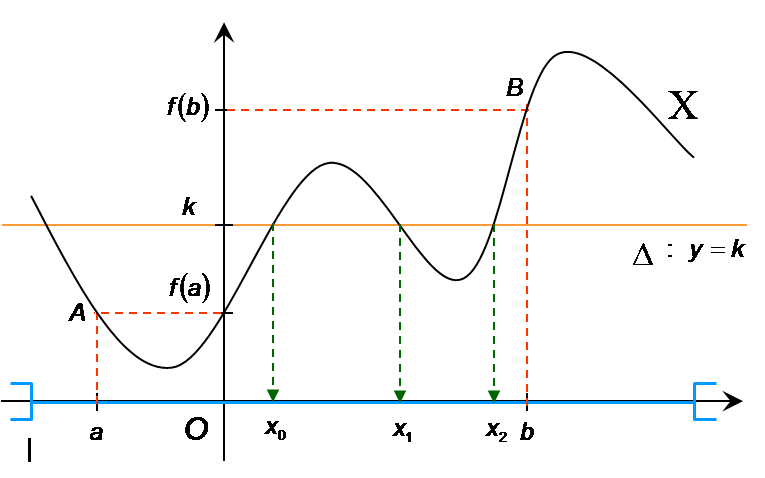
\includegraphics[scale=0.6]{images/001.png}
\end{center}

\subsection{Preuve}
Soient $a,b \in I$ et $\alpha=f(a)$ et $\beta=f(b)$, supposons $a<b$ et $\alpha<\beta$ (réciproquement $\alpha>\beta$).
Soit $y\in ]\alpha,\beta[$, montrons que y possède un antécédent dans [a;b].\\\\
Soit $E=\{x\in[a;b] | f(x)\leq y\}$, $a\in E$, E est majoré par b et donc admet une borne supérieure $x_{0}$.

$\exists (U_{n})_{n\in\N}\subset E$ qui converge vers $x_{0}$. Comme $f$ est continue en $x_{0}$, la suite $f(U_{n})$ converge vers $f(x_{0})$ et comme $\forall n\in\N$, $f(U_{n})\leq y$, on a $f(x_{0})\leq y$.\\

Puisque f(b)>y, on a $x_{0}\neq b$ or $\forall x\in ]x_{0};b[$, $f(x)>y$ d'où la limite à droite de $f$ en $x_{0}$ (égale à $f(x_{0})$ car $f$ continue en $x_{0}$) est supérieure ou égale à y, c'est-à-dire $f(x_{0})\geq y$.\\

D'où finalement $f(x_{0})=y$

\subsubsection{Remarque}
La réciproque du théorème des valeurs intermédiaires est fausse. Il existe des fonctions discontinues qui possèdent la propriété des valeurs intermédiaires.

\subsection{Corollaire}
Soit $f : D_{f}\rightarrow \R$ continue et $I$ inclue dans $D_{f}$ un intervalle, alors f(I) est un intervalle.

\subsubsection{Preuve}
$\forall \alpha,\beta \in f(I)$, on a que $\forall y\in ]\alpha;\beta[$, $y\in f(I)$ d'après le théorème des valeurs intermédiaires,\\
donc $]\alpha;\beta[\subset f(I)$ et donc f(I) est un intervalle.

\subsubsection{Exemples}
\begin{enumerate} \item Soit $f:\begin{array}{rcl} \R^{*}&\rightarrow& \R \\
x&\mapsto &\frac{1}{x} \end{array}$. $f(]0;1])=[1;+\infty[$.

\item Soit $g:\begin{array}{rcl} \R&\rightarrow& [-1;1] \\
x&\mapsto& sin(x) \end{array}$. $g(]0;2\pi[)=[-1;1]$. \end{enumerate}

\subsubsection{Remarque}
L'image d'un ensemble ouvert par une fonction continue n'est pas nécessairement ouvert et l'image d'un intervalle borné par une fonction continue n'est pas nécessairement bornée.

\newpage

\subsection{Théorème de Weierstrass ou théorème des bornes atteintes}
\subsubsection{Énoncé}
Une fonction continue sur un segment [a;b] est bornée et atteint des bornes, c'est-à-dire que l'image d'un segment par une fonction continue est un segment.

Soit $f:D_{f}\rightarrow \R$ continue et $[a;b]\subset D_{f}$, $f([a;b])=\left[\underset{x\in [a;b]}{inf(f(x))};\underset{x\in [a;b]}{sup(f(x))}\right]$.

\subsubsection{Preuve}
Soit $J=f([a;b])$ et $M=sup(J)$, si J est majoré alors $M\in \R$ $(M\neq +\infty)$ sinon $M=+\infty$.\\

Tout d'abord d'après le corollaire, J est un intervalle. Il faut donc montrer que $M\neq +\infty$ et que $M\in J$ (de façon analogue on montre que $m=inf(J)\neq -\infty$ et $m\in J$).\\

$\exists (y_{n})_{n\in\N}\subset J$ convergeant vers M si $M\in \R$ et divergeant si $M=+\infty$
(par abus de notation on dira dans les deux cas que $\lim\limits_{n\rightarrow +\infty} y_{n}=M)$.\\

$\forall n\in \N$, $y_{n}\in f([a;b])$ donc d'après le \tvi,\\
$\exists x_{n}\in [a;b]$ tel que $f(x_{n})=y_{n}$.\\

La suite $(x_{n})_{n\in \N}$ est bornée, on peut donc en extraire une suite convergente $(x_{\phi(n)})_{n\in\N}$\\
($\phi:\N\rightarrow\N$ strictement croissante).\\

On pose $\lim\limits_{n\rightarrow +\infty} x_{\phi(n)}=l$, $(x_{\phi(n)})_{n\in\N}$ étant définie sur le segment [a;b] (fermé), $l\in [a;b]$.\\

Comme $f$ est continue sur $[a;b]$ et donc en l, on a que $f(x_{\phi(n)})=y_{\phi(n)}$ converge vers f(l)\\
avec f(l) une limite finie. Ainsi on peut extraire de $(y_{n})_{n\in\N}$, une sous-suite $(y_{\phi(n)})_{n\in\N}$ convergente.\\

Alors $(y_{n})_{n\in\N}$ ne diverge pas vers $+\infty$. En effet on a $\lim\limits_{n\rightarrow +\infty} y_{n}=M=\lim\limits_{n\rightarrow +\infty} y_{\phi(n)}=f(l)$\\
et donc M=f(l) est fini ($\neq +\infty$) et $M\in J=f([a,b]$) car $f$ continue en $l\in [a;b]$.\\

Finalement, J est majoré et sa borne supérieure est atteinte; de la même façon, on a que J est minoré et sa borne inférieure est atteinte.

\subsection{Propositions}
\subsubsection{Énoncés}
Soit $f :I\rightarrow \R$ une fonction continue,
\begin{enumerate} \item Si $f$ est injective alors elle est strictement monotone.\\

Si $f$ est strictement monotone,
\item f(I) est un intervalle dont les bornes sont les limites de $f$ aux bornes de I.
\item $f$ est une bijection de $I$ dans f(I).
\item Sa bijection réciproque est continue sur f(I) et strictement monotone de même sens que f.\end{enumerate}

\subsubsection{Démonstrations}
\begin{enumerate} \item
\begin{enumerate}
\item Supposons $f$ non monotone, $\exists (a;b;c) \in I^{3}$ tels que $a<b<c$, $f(a)<f(b)$ et
$f(c)<f(b)$ (c'est-à-dire $\exists J\in I$ tel que $f$ ou $-f$ est croissante puis décroissante sur J).\\

Soit $y\in \left[max(f(a),f(c));f(b)\right[$, d'après le \tvi, $y$ a un\\
antécédent dans $[a;b[$ et dans $]b;c]$ donc $\exists x_{1},x_{2}$ tels que $x_{1}\neq x_{2}$ mais $f(x_{1})=f(x_{2})=y$ donc $f$ n'est pas injective.\\

\item Supposons $f$ monotone non strictement, $\exists J\subset I$ tel que l'intervalle J contient\\
au moins 2 points et $f$ est constante sur J.\\

Soient $x_{1}\neq x_{2} \in J\subset I$ on a $f(x_{1})=f(x_{2})$ donc $f$ n'est pas injective.\\ \end{enumerate}

\item $\forall x_{0} \in$ $]a;b[$ on a $\lim\limits_{x\rightarrow a}f(x)<f(x_{0})<\lim\limits_{x\rightarrow b}f(x)$ car $f$ est strictement croissante,\\
donc $f(I)\subset \left]\lim\limits_{x\rightarrow a}f(x) ; \lim\limits_{x\rightarrow b}f(x) \right[$.\\

D'autre part, soit $y\in \left]\lim\limits_{x\rightarrow a}f(x) ; \lim\limits_{x\rightarrow b}f(x) \right[$. y n'est ni un majorant ni un minorant de f(I) donc il existe $x_{1},x_{2}\in I^{2}$ tels que 
$f(x_{1})<y<f(x_{2})$.\\

D'après le \tvi, il existe $x_{0} \in I$ tel que $f(x_{0})=y$ donc $y\in f(I)$, c'est-à-dire que $\left]\lim\limits_{x\rightarrow a}f(x) ; \lim\limits_{x\rightarrow b}f(x) \right[\subset f(I)$.\\

Finalement, $f(I)=\left]\lim\limits_{x\rightarrow a}f(x) ; \lim\limits_{x\rightarrow b}f(x) \right[$.\\

\item Par définition $f$ est surjective dans f(I). On veut donc montrer que $f$ est injective:\\

Soient $x_{1},x_{2} \in I^{2}$ tels que $f(x_{1})=f(x_{2})$.\\

Si $x_{1}<x_{2}$, $f(x_{1})<f(x_{2})$ car $f$ est strictement croissante, ce qui est impossible.\\
Si $x_{1}>x_{2}$, $f(x_{1})>f(x_{2})$ car $f$ est strictement croissante, ce qui est impossible.\\

Donc $x_{1}=x_{2}$.

\item Soient $y_{1},y_{2}\in f(I)$, on suppose $y_{1}<y_{2}$ et on pose $x_{1}=f^{-1}(y_{1})$ et $x_{2}=f^{-1}(y_{2})$.\\

\begin{tikzpicture}[scale=1.5]
\draw[->] (0,0) -- (3.75,0);
\draw[->] (0,0) -- (0,4);
\node[scale=0.8] at (3.75,-0.15) {$x$} ;
\node[scale=0.8] at (-0.2,4) {$y$} ;

\draw [domain=0.5:3.5, samples=100] plot (\x,{-0.13*\x*\x +1.5*\x}) ;

\draw[very thin, densely dashed] (0,3.2) -- (2.82,3.2) ;
\draw[very thin, densely dashed] (0,3) -- (2.6,3) ;
\draw[very thin, densely dashed] (0,2.8) -- (2.35,2.8) ;

\draw[very thin, densely dashed] (2.82,0) -- (2.82,3.2) ;
\draw[very thin, densely dashed] (2.6,0) -- (2.6,3) ;
\draw[very thin, densely dashed] (2.35,0) -- (2.35,2.8) ;

\node[scale=0.8] at (-0.2,3) {$y_{0}$} ;
\node[scale=0.8] at (-0.2,3.2) {$y_{2}$} ;
\node[scale=0.8] at (-0.2,2.8) {$y_{1}$} ;

\node[scale=0.8] at (2.88,-0.15) {$x_{2}$} ;
\node[scale=0.8] at (2.62,-0.15) {$x_{0}$} ;
\node[scale=0.8] at (2.35,-0.15) {$x_{1}$} ;

\draw[very thick, <->] (0.8,0) -- (3.4,0) ;
\node[thick] at (1.5,0.2) {I} ;

\draw[very thin, densely dashed] (0.8,1.12) -- (0.8,-0.05) node[below, scale=0.8] {$a$} ;
\draw[very thin, densely dashed] (3.4,3.59) -- (3.4,-0.05) node[below, scale=0.8] {$b$} ;
\draw[very thin, densely dashed] (0.8,1.12) -- (-0.05,1.12) node[left, scale=0.8] {$f(a)$} ;
\draw[very thin, densely dashed] (3.4,3.59) -- (-0.05,3.59) node[left, scale=0.8] {$f(b)$} ;

\draw[<->, very thin] (2.6,0.3) -- (2.82,0.3) node[scale=0.6,midway, below] {$+\epsilon$} ;
\draw[<->, very thin] (2.6,0.3) -- (2.35,0.3) node[scale=0.6,midway, below] {$-\epsilon$} ;

\node at (-4,4) {Si $x_{1}\geq x_{2}$ alors $f(x_{1})\geq f(x_{2})$, ce qui est impossible, donc $x_{1}<x_{2}$} ;
\node at (-5.625,3.73) {donc $f^{-1}$ est strictement croissante.} ;
\node at (-4.55,3.16) {On veut montrer que $f^{-1}$ est continue, on pose $I=]a;b[$.} ;
\node at (-4.95,2.6) {Soient $y_{0}\in f(I)$  $\left(f(I)=D_{f^{-1}}\right)$ et $x_{0}=f^{-1}(y_{0})$.} ;
\node at (-5.28,2.3) {Soit $\epsilon>0$ tel que $x_{0}-\epsilon\in I$ et $x_{0}+\epsilon\in I$.} ;
\node at (-5.4,1.725) {Posons $y_{1}=f(x_{0}-\epsilon)$ et $y_{2}=f(x_{0}+\epsilon)$.} ;
\node at (-4.2,1.15) {f strictement croissante donc $y_{1}<y_{0}<y_{2}$ et donc $\forall y\in [y_{1};y_{2}]$,} ;
\node at (-3.85,0.85) {$f^{-1}(y_{1})\leq f^{-1}(y)\leq f^{-1}(y_{2})$ c'est-à-dire que $x_{0}-\epsilon\leq f^{-1}(y)\leq x_{0}+\epsilon$.} ;
\node at (-4.45,0.2) {Ainsi $\exists\eta>0$ tel que $|y-y_{0}|\leq \eta \Rightarrow |f^{-1}(y)-f^{-1}(y_{0})|\leq \epsilon$} ;
\node at (-5.8,-0.1) {d'où $f^{-1}$ est continue $\forall y\in f(I)$.} ;
\end{tikzpicture}
\end{enumerate}
\bigskip
\subsection{Remarque}
Soit $C_{f}$ la courbe représentative de f, une fonction continue strictement monotone. La courbe représentative de $f^{-1}$ est symétrique à $C_{f}$ par rapport à la première diagonale (y=x).


% ------------------------------------------------------------------------------------------------------ %
% ------------------------------------------------------------------------------------------------------ %



% ------------------------------------------------------------------------------------------------------ %
% ------------------------------------------------------------------------------------------------------ %


\chapter{Fonctions dérivables}
\section{Généralités}
\subsection{Définition}
Soit $f : I\subseteq\R \rightarrow \R$, $x_{0}\in I$, $f$ est dérivable si et seulement si la fonction $x\mapsto \frac{f(x)-f(x_{0})}{x-x_{0}}$ admet une limite finie quand x tend vers $x_{0}$.\\

Quand la fonction est dérivable, on note $f'(x_{0})$ la dérivée de $f$ en $x_{0}$ et $f'(x_{0})=\lim\limits_{x\rightarrow x_0}\frac{f(x)-f(x_{0})}{x-x_{0}}$.

\subsubsection{Proposition}
Toute fonction dérivable en $x_{0}$ est continue en $x_{0}$.

\subsubsection{Preuve}
Si une fonction $f$ est dérivable en $x_{0}$ alors $\lim\limits_{x\rightarrow x_0}\frac{f(x)-f(x_{0})}{x-x_{0}}$ existe et est finie.\\
La limite de $f(x)$ en $f(x_{0})$ est $0$ car sinon $\lim\limits_{x\rightarrow x_0}\frac{f(x)-f(x_{0})}{x-x_{0}}=\pm\infty$.

On a donc $\lim\limits_{x\rightarrow x_{0}} f(x)=f(x_{0})$ et donc $f$ est continue en $x_{0}$.

\subsubsection{Remarque}
La réciproque est fausse : la fonction valeur absolue n'est pas dérivable en 0.\\

En effet, $\frac{|x|-|0|}{x-0}=\frac{|x|}{x}$ n'admet pas de limite en 0 ($\lim\limits_{x\rightarrow 0^{+}} \frac{|x|}{x}=1$ et $\lim\limits_{x\rightarrow 0^{-}} \frac{|x|}{x}=-1$).


\subsection{Dérivabilité à gauche et à droite}
Il est parfois nécessaire de définir une notion de dérivabilité à gauche et à droite.

\subsubsection{Définition}
Une fonction $f:I\rightarrow \R$ est dérivable à droite (resp à gauche) en $x_{0}$ si et seulement si la restriction de $f$ à $I\cap [x_{0};+\infty]$ (resp $I\cap ]-\infty;x_{0}])$ est dérivable en $x_{0}$.\\

En d'autre termes, $f$ est dérivable à droite en $x_{0}$ (respectivement à gauche) si et seulement\\
si $x\mapsto \frac{f(x)-f(x_{0})}{x-x_{0}}$ admet une limite finie à droite en $x_{0}$ (respectivement limite à gauche).

\subsection{Dérivabilité sur un intervalle}
Une fonction $f : I\subseteq \R \rightarrow \R$ est dérivable sur $A\subseteq I$ si et seulement si la restriction de $f$ à A est dérivable en tout point de A.\\

On peut définir la fonction dérivée de $f$ sur A comme $f' : \begin{array}{rcl}
A&\rightarrow& \R \\
x&\mapsto& f'(x) \end{array}$.

\subsubsection{Remarque}
Soient $f : I\subseteq \R \rightarrow \R$ et $[a;b] \subset I$, $f$ peut être dérivable sur $[a;b]$ sans être dérivable en a.\\

$f|_{[a;b]}$ dérivable en a signifie que $f$ est dérivable à droite en a, alors que $f$ dérivable en a signifie que les dérivées à gauche et à droite sont égales.\\

Par exemple la fonction valeur absolue n'est pas dérivable en 0 mais $f|_{\R^{+}}$ est dérivable en 0.\\
Donc $f$ n'est pas dérivable sur $\R$ mais est dérivable sur $\R^{+}$.

\subsection{Dérivées usuelles}
\begin{enumerate}
\item Une fonction constante est dérivable sur $\R$ et la dérivée de $f(x)=a$, $a\in \R$ est $f'(x)=0$.\\

\emph{Preuve :}\\
Soit $x_{0}\in \R$, $\frac{f(x)-f(x_{0})}{x-x_{0}}=\frac{a-a}{x-x_{0}}=0$ si $x\neq x_{0}$ donc $\lim\limits_{x\rightarrow x_{0}}\frac{f(x)-f(x_{0})}{x-x_{0}}$ existe et vaut 0.\\\\

\item La fonction identité est dérivable sur $\R$ et la dérivée de $f(x)=x$ est $f'(x)=1$.\\

\emph{Preuve :}\\
$\frac{f(x)-f(x_{0})}{x-x_{0}}=\frac{x-x_{0}}{x-x_{0}}=1$ si $x\neq x_{0}$ donc $\lim\limits_{x\rightarrow x_{0}}\frac{f(x)-f(x_{0})}{x-x_{0}}$ existe et vaut 1.\\\\

\item La fonction inverse est dérivable sur $\R^*$ et la dérivée de $f(x)=\frac{1}{x}$ est $f'(x)=\frac{1}{x^2}$.\\

\emph{Preuve :}\\
Soit $x_{0}\in \R^{*}$, $\frac{f(x)-f(x_{0})}{x-x_{0}}=\frac{\frac{1}{x}-\frac{1}{x_{0}}}{x-x_{0}}
=\frac{\frac{x_0-x}{xx_0}}{x-x_0}=\frac{-1}{xx_{0}}$, donc la limite est finie quand x tend vers $x_{0}$ ($x_0\neq 0$) et vaut $\frac{-1}{x^{2}}$.
\end{enumerate}

\newpage

\section{Interprétations et notations}
\subsection{Notations}
La fonction dérivée de $f$ est parfois notée f', Df ou encore $\frac{df}{dx}$ (notation de Leibniz) qui rappelle que la dérivée est la limite du taux d'accroissement $\frac{\Delta f}{\Delta x}$ quand $\Delta x$ tend vers 0.\\

\subsection{Interprétation géométrique}
\begin{wrapfigure}[10]{r}{3cm}
\begin{tikzpicture}[scale=0.8]
\draw[->] (0,0) -- (5,0) node[above] {x};
\draw[->] (0,0) -- (0,5) node[below right] {y};
\draw [domain=0:4.25, samples=100] plot (\x,{\x^2/4}) ;
\draw[densely dashed, thin] (2,1) -- (0,1) node[left, scale=0.75] {$x_0$} ;
\draw[densely dashed, thin] (2,1) -- (2,0) node[below, scale=0.75] {$f(x_0)$} ;
\draw[densely dashed, thin] (4,4) -- (0,4) node[left, scale=0.75] {$x$} ;
\draw[densely dashed, thin] (4,4) -- (4,0) node[below, scale=0.75] {$f(x)$} ;
\node[scale=0.85] at (1.85,1.25) {$A_0$} ;
\node[scale=0.85] at (3.85,4.25) {$A$} ;
\draw[very thin, densely dashed] (1.33,0) -- (4.5,4.75) ;
\end{tikzpicture}
\end{wrapfigure}

Le quotient $\frac{f(x)-f(x_{0})}{x-x_{0}}$ représente le taux d'accroissement de la fonction $f$ entre $x$ et $x_{0}$. C'est le coefficient directeur de la droite reliant les points de la courbe $C_{f}$ représentative de $f$ d'abscisse $x$ et $x_{0}$, c'est-à-dire $A(x;f(x))$ et $A_{0}(x_{0};f(x_{0}))$.

\bigskip

f est dérivable signifie que la droite $(A_{0},A)$ a une position limite lorsque A "tend vers" $A_{0}$ (de n'importe quel côté de $A_{0}$ mais en restant sur $C_{f}$).\\

La droite de position limite est appelée tangente à $C_{f}$ en $A_{0}$.\\
La dérivée $f'(x_{0})$ est le coefficient directeur de cette tangente.

\subsubsection{Équation de la tangente}
Soient $C_{f}$ la courbe représentative d'une fonction $f : I\rightarrow \R$, $x_{0}\in I$ et $A_{0}(x_{0};f(x_{0}))\in C_{f}$.\\
Une équation de la tangente à $C_{f}$ en $A_{0}$ (lorsque celle-ci existe) est $y-f(x_{0})=f'(x_{0})(x-x_{0})$.

\subsection{Interprétation cinématique}
Si $f(t)$ représente la position à l'instant t d'un mobile sur un axe, le quotient $\frac{f(t)-f(t_{0})}{t-t_{0}}$ représente la vitesse moyenne du mobile entre les temps $t_{0}$ et $t$.\\

La dérivée $f'(t_{0})$, si elle existe, représente ainsi la vitesse instantanée du mobile à l'instant $t_{0}$.

\subsubsection{Remarque}
De la même façon, on peut associer la notion mathématique de dérivée à celle d'accélération d'un mobile (dérivée de la vitesse).

\subsection{Applications}
A ce stade on peut dégager plusieurs applications de la dérivée:
\begin{enumerate}
\item Étude de variations de fonctions.
\item Recherche d'extremums d'une fonction (tangentes horizontales) et donc optimisation\\
de fonctions.
\item Approximation affine locale d'une fonction.
\item Étude de la convexité d'une courbe (position relative de la courbe par rapport à la tangente).
\end{enumerate}

\subsection{Dérivées successives}
Si $f$ est n fois dérivable, on note $f^{(n)}$ sa dérivée d'ordre n (n-ième) et on dit que $f$ est de classe $C^{n}$ sur $I$ si elle admet une dérivée d'ordre n sur $I$ et que $f^{(n)}$ est continue.\\

$C^{\infty}$ est l'ensemble des fonctions admettant une dérivée de tout ordre (nécessairement continue) car dérivable.\\

Lorsque $n=2$ on notera $f^{(2)}=f''$.

\newpage

\section{Opérations sur les dérivées}
Soient $f$ et $g$ deux fonctions dérivables sur $I\subseteq \R$.
\subsection{Somme}
\subsubsection{Énoncé}
$(f+g)$ est dérivable sur $I$ et $(f+g)'=f'+g'$.

\subsubsection{Démonstration}
Soit $x_{0}\in I$, $\frac{(f+g)(x)-(f+g)(x_{0})}{x-x_{0}}=\frac{f(x)-f(x_{0})}{x-x_{0}}+\frac{g(x)-g(x_{0})}{x-x_{0}}$ or $f$ et $g$ sont dérivables sur I\\
donc $\frac{f(x)-f(x_{0})}{x-x_{0}}+\frac{g(x)-g(x_{0})}{x-x_{0}}=f'(x_{0})+g'(x_{0})=(f'+g')(x_{0})$.

\subsection{Produit}
\subsubsection{Énoncé}
$fg$ est dérivable sur $I$ et $(fg)'=f'g+g'f$.

\subsubsection{Démonstration}
Soit $x_{0}\in I$, $\frac{(fg)(x)-(fg)(x_{0})}{x-x_{0}}=\frac{f(x)g(x)-f(x_{0})g(x)+f(x_{0})g(x)-f(x_{0})g(x_{0})}{x-x_{0}}=\frac{g(x)(f(x)-f(x_{0}))}{x-x_{0}}+\frac{f(x)(g(x)-g(x_{0}))}{x-x_{0}}$.\\

On a :\begin{enumerate}
\item $\lim\limits_{x\rightarrow x_{0}}g(x)=g(x_{0})$ car $g$ dérivable en $x_{0}$ donc $g$ continue en $x_0$.
\item $\lim\limits_{x\rightarrow x_{0}}f(x_{0})=f(x_{0})$ car $f(x_{0})$ est une constante.
\item $\lim\limits_{x\rightarrow x_{0}}\frac{f(x)-f(x_{0})}{x-x_{0}}=f'(x_{0})$ par hypothèse.
\item $\lim\limits_{x\rightarrow x_{0}}\frac{g(x)-g(x_{0})}{x-x_{0}}=g'(x_{0})$ par hypothèse.
\end{enumerate}

Ainsi $fg$ est dérivable en $x_0$ et $(fg)'(x_0)= \lim\limits_{x\rightarrow x_{0}}\frac{(fg)(x)-(fg)(x_{0})}{x-x_{0}}=(f'g)(x_{0})+(g'f)(x_0)$.

\subsubsection{Corollaire}
Soit $f_a : x\mapsto x^a$ avec $a\in \N^{*}$, $f_a$ est dérivable sur $\R$ et $f'_a : x\mapsto ax^{a-1}$.

\subsubsection{Preuve}
On va procéder par récurrence, on appelle $P_n$ la proposition "$(x^n)'=nx^{n-1}$".\\

\emph{Initialisation :}\\
Pour $n=1$, on a $f(x)=x$ et $f'(x)=1=1\times x^0$ donc $P_0$ est vraie.\\

\emph{Hérédité :}\\
Supposons $f'_n : x \mapsto nx^{n-1}$, $f_{n+1}(x)=x^{n+1}=x\times x^{n}$, donc $f_{n+1}=x\times f_n$ et donc\\
$(f_{n+1})'=xf_n'+x'f_n=nx^n+x^n=(n+1)x^{n}$ donc $P_n$ est héréditaire.\\

Ainsi $P_n$ est initialisable et héréditaire, donc $P_n$ est vraie pour tout $n\in \N^*$ et donc\\
$f'_{a} : x\mapsto ax^{a-1}$.

\newpage

\subsection{Fonction composée}
\subsubsection{Proposition}
Si $f$ est dérivable sur $I\subseteq \R$ et $g$ dérivable sur $f(I)$, alors la fonction $g\circ f$ est dérivable\\
sur $I$ et $g(f(x))'=f'(x)\times g'(f(x))$.

\subsubsection{Preuve}
On a $\frac{g(f(x_{0})+f(x)-f(x_{0}))-g(f(x_{0}))}{x-x_{0}}=\frac{g(f(x_{0})+f(x)-f(x_{0}))-g(f(x_{0}))}{f(x)-f(x_0)} \times \frac{f(x)-f(x_{0})}{x-x_{0}}$.\\

Or $g$ est dérivable sur $f(I)$ donc en $f(x_0)$, donc en posant $h(x)=f(x)-f(x_0)$ on a que\\
$\lim\limits_{x\rightarrow x_0}\frac{g(f(x_{0})+h(x))-g(f(x_{0}))}{h(x)}$ est finie et vaut $(g\circ f)'(x_0)$ (car $f$ est dérivable en $x_{0}$ donc $f$ est continue en $x_0$ et donc $\lim\limits_{x\rightarrow x_0}f(x)-f(x_{0})=\lim\limits_{x\rightarrow x_0} h(x)=0$).\\

De plus $\lim\limits_{x\rightarrow x_0}\frac{f(x)-f(x_{0})}{x-x_{0}}=f'(x_0)$ puisque $f$ est dérivable en $x_0$.\\

Ainsi $(g\circ f)'(x_0)$ est dérivable en $x_0$ et\\
$(g\circ f)'(x_0)=\lim\limits_{x\rightarrow x_0}\frac{g(f(x_{0})+f(x)-f(x_{0}))-g(f(x_{0}))}{f(x)-f(x_0)} \times \frac{f(x)-f(x_{0})}{x-x_{0}}=f'(x_0)\times g'(f(x_0))$.

\subsection{Quotient de fonctions}
\subsubsection{Proposition}
Si $g$ ne s'annule pas sur I, alors $\frac{1}{g}$ et $\frac{f}{g}$ sont dérivables sur $I$ et $(\frac{1}{g})'=\frac{-g}{g^{2}}$ et $(\frac{f}{g})'=\frac{f'g-g'f}{g^{2}}$.

\subsubsection{Preuve}
Soit $u:x\mapsto \frac{1}{x}$ alors $\frac{1}{g}=u\circ g$ et donc $(\frac{1}{g})'=(u\circ g)'=g'\times u'\circ g=\frac{-g'}{g^{2}}$.\\

$(\frac{f}{g})'=(f\times \frac{1}{g})'=\frac{f'}{g}+f\times (\frac{1}{g})'=\frac{f'}{g}-\frac{fg'}{g^{2}}=\frac{f'g-g'f}{g^{2}}$\\

\subsubsection{Corollaire}
Soit $f_{-a}(x)=x^{-a}$ avec $a\in \N$, $f$ est dérivable sur $\R^{*}$ et $f'_{-a}(x)=-ax^{-a-1}$.\\

On peut généraliser ce résultat à $f_a(x)=x^{a}$ pour $a \in \R$.\\
$f_a$ est dérivable sur $\R$ si $a\geq 0$ et sur $\R^{*}$ sinon et $f'_a(x)=x^{a-1}$.\\

\subsection{Dérivée d'une fonction réciproque}
Si $f$ est une fonction bijective et dérivable sur $I$ alors sa réciproque $f^{-1}$ est dérivable sur $f(I)$ et si f' ne s'annule pas sur f(I) alors $(f^{-1})'=\frac{1}{f\circ f^{-1}}$.

\subsubsection{Preuve}
$(f^{-1})'(y_{0})=\lim\limits_{y \rightarrow y_{0}}\frac{f^{-1}(y)-f^{-1}(y_{0})}{y-y_{0}}$ or $\frac{f^{-1}(y)-f^{-1}(y_{0})}{y-y_{0}}=\frac{f^{-1}(y)-f^{-1}(y_{0})}{f(f^{-1}(y))-f(f^{-1}(y_{0}))}\\
\hspace*{8.2cm}=\frac{1}{\frac{f(f^{-1}(y))-f(f^{-1}(y_{0}))}{f^{-1}(y)-f^{-1}(y_{0})}}$\\\\

donc $(f^{-1})'(y_{0})=\lim\limits_{y \rightarrow y_{0}} \frac{f^{-1}(y)-f^{-1}(y_{0})}{y-y_{0}}=\frac{1}{f'(f^{-1}(y_{0}))}$.

\newpage

\section{Extremums locaux}
\subsection{Définition}
Soient $f : D_{f} \subseteq \R \rightarrow \R$ et $x_{0}\in D_f$,
\begin{enumerate}
\item $x_{0}$ est un maximum local si et seulement si $\exists \alpha>0$ tel que $\forall x\in ]x_{0}-\alpha;x_{0}+\alpha[$,\\
on a $x\in D_f$ et $f(x)\leq f(x_0)$.

\item $x_{0}$ est un minimum local si et seulement si $\exists \alpha>0$ tel que $\forall x\in ]x_{0}-\alpha;x_{0}+\alpha[$,\\
on a $x\in D_f$ et $f(x)\geq f(x_0)$.
\end{enumerate}

\subsubsection{Remarque}
Les bornes peuvent être des bornes supérieures ou inférieures de $f$ sans être des extremum locaux.\\

\emph{Exemple :}\\
Soit $f(x)=x$ sur $I=[0;1]$, 0 et 1 sont respectivement les bornes inférieures et supérieures de $f$ mais ne sont pas des extremums locaux.

\subsection{Théorème}
\subsubsection{Énoncé}
Soient $f : D_f \subseteq \R \rightarrow \R$ et $x_0 \in D_f$. Si $f$ est dérivable en $x_0$ alors $x_0$ est un extremum local implique que $f'(x_0)=0$.

\subsubsection{Preuve}
Supposons que $x_0$ est un maximum local de f, $\exists \alpha>0$ tel que $\forall x\in ]x_{0}-\alpha;x_{0}+\alpha[$,\\
$x\in D_f$ et $f(x)\leq f(x_0)$.\\

$\forall x_1\in ]x_{0}-\alpha;x_{0}[$, $\frac{f(x_1)-f(x_0)}{x_1-x_0}\geq 0$ donc $\lim\limits_{x_1\rightarrow x_0^-}\frac{f(x_1)-f(x_0)}{x_1-x_0}=f'(x_0)\geq 0$ (car $f$ dérivable en $x_0$).\\

Réciproquement dans la partie droite de l'intervalle on trouve $f'(x_0)\leq 0$ et\\
donc finalement $f(x_0)=0$.

\subsubsection{Réciproque}
La réciproque est fausse : prenons $f(x)=x^3$ sur $\R$, $f'(x)=3x^2$ donc f'(0)=0 mais 0 n'est pas un extremum local.

\subsubsection{Remarque}
Graphiquement la courbe représentative d'une fonction dérivable admet des tangentes horizontales en ses extremums locaux (équation de la tangente).

\newpage

\section{Fonctions usuelles}
\subsection{Fonction exponentielle}
Par définition, la fonction exponentielle $exp: \begin{array}{rcl}
\R & \rightarrow & \Rpe \\
x&\mapsto & \exp(x) \end{array}$ est dérivable sur $\R$ et est invariante par la dérivation : $\exp'(x)=\exp(x)$.

\subsection{Logarithme népérien}
La fonction exponentielle est bijective de $\R$ dans $\Rpe$ et sa bijection réciproque est le logarithme népérien $\ln:\begin{array}{rcl}
\Rpe & \rightarrow & \R \\
x & \mapsto & ln(x) \end{array}$\\

Ainsi $\ln$ est dérivable sur $\Rpe$ (dérivabilité de la fonction réciproque) et $\ln'(x)=\frac{1}{\exp'(ln(x))}=\frac{1}{x}$.

\subsection{Sinus}
\subsubsection{Proposition}
La fonction sinus est dérivable sur $\R$ et $\sin'(x)=\cos(x)$.

\subsubsection{Démonstration}
On a $\frac{\sin(x+h)-\sin(x)}{h}=\frac{\sin(x)\cos(h)+\sin(h)\cos(x)-\sin(x)}{h}= \sin(x)\frac{\cos(h)-1}{h}+\cos(x)\frac{\sin(h)}{h}$.\\

\begin{tikzpicture}
\draw (0,0) circle (2) ;
\draw[->] (0,-2.25) -- (0,2.5);
\draw[->] (-2.25,0) -- (2.5,0) ;
\node at (-0.2,-0.2) {O} ;
\node at (2.2,-0.2) {A} ;
\node at (1,-0.2) {c} ;
\draw[->] (2,-2.25) -- (2,2.5) ;
\node at (3.15,0) {$\cos(x)$} ;
\node at (0.2,2.75) {$\sin(x)$} ;
\node at (2,2.75) {$\tan(x)$} ;
\draw[thick] (0.3,0) arc (0:45:0.3) ;
\draw (0,0) -- (2.3,2.3) ;
\node at (2.2,1.9) {D} ;
\node[scale=0.9] at (0.42,0.17) {\textbf{h}};
\draw[densely dashed, very thin] (0,1.414)--(1.414,1.414) ;
\draw[densely dashed, very thin] (2,0) -- (1.414,1.414);
\foreach \x in {0.05,0.15,0.25,...,2.05} {\draw[very thin] (\x,0) -- (0.7*\x,0.7*\x); }
\draw[very thin] (2,0.13) -- (1.473,1.35) ;
\draw[very thin] (1.935,0.5) -- (1.7,1.05);
\node at (1.42,1.65) {B} ;
\node at (-5,0) {On suppose $h\in ]-\frac{\pi}{2};\frac{\pi}{2}[$ :} ;
\end{tikzpicture}

On note $\wideparen{AOB}$ la portion du disque trigonométrique entre O, A et B (zone hachurée).\\

On a $\mathcal{A}(\wideparen{AOB})=\frac{|h|\pi}{2\pi}=\frac{|h|}{2}$, $\mathcal{A}(AOB)=\frac{|\sin(h)|}{2}$ et $\mathcal{A}(AOD)=\frac{|\tan(h)|}{2}$, et donc alors\\
$\mathcal{A}(AOB)\leq \mathcal{A}(\wideparen{AOB})\leq \mathcal{A}(AOD)$ donc $\frac{|\sin(h)|}{2}\leq \frac{|h|}{2} \leq \frac{|\tan(h)|}{2}$ et enfin $|\sin(h)|\leq |h| \leq |\tan(h)|$.\\\\
On a donc $\frac{1}{|\sin(h)|}\geq \frac{1}{|h|}\geq \frac{\cos(h)}{|\sin(h)|}$ $\Leftrightarrow$ $1\geq |\frac{\sin(h)}{h}|=\frac{\sin(h)}{h}\geq \cos(h)$ ($\sin(h)$ et h sont de même signe)\\

On applique le théorème des gendarmes : $\lim\limits_{h\rightarrow 0}\frac{\sin(h)}{h}=1$.\\

D'autre part : $\frac{\sin(h)}{h}=\frac{\sin^{2}(h)}{h\times \sin(h)}=\frac{1-\cos{2}(h)}{h\times \sin(h}=\frac{1-\cos(h)}{|h|} \times \frac{1+\cos(h)}{|\sin(h)|}$\\

or $\lim\limits_{h\rightarrow 0} \frac{1+\cos(h)}{|\sin(h)|}=+\infty$ et $\lim\limits_{h\rightarrow 0}\frac{1-\cos(h)}{|h|}\times \frac{1 +\cos(h)}{|\sin(h)|}=\lim\limits_{h\rightarrow 0}\frac{\sin(h)}{h}=1$.\\\\\\
Supposons $\lim\limits_{h\rightarrow 0} \frac{1-\cos(h)}{|h|}\neq 0$ alors $\lim\limits_{h\rightarrow 0}\frac{\sin(h)}{h}=\pm \infty$ ce qui est impossible car $\lim\limits_{h\rightarrow 0}\frac{\sin(h)}{h}=1$.\\
Donc $\lim\limits_{h \rightarrow 0} \frac{1-\cos(h)}{|h|}=0=\lim\limits_{h\rightarrow 0}\frac{\cos(h)-1}{h}$.\\

Finalement $\lim\limits_{h\rightarrow 0} \frac{\sin(x+h)-\sin(x)}{h}=\cos(x)$.

\newpage	

\subsection{Cosinus}
\subsubsection{Proposition}
La fonction cosinus est dérivable sur $\R$ et $\cos'(x)=-\sin(x)$.

\subsubsection{Preuve}
$\frac{\cos(x+h)-\cos(x)}{h}=\frac{\cos(x)\cos(h)-\sin(x)\sin(h)-\cos(x)}{h}=\cos(x)\frac{\cos(h)-1}{h}-\sin(x)\frac{\sin(h)}{h}$\\\\
d'où $\lim\limits_{h \rightarrow 0}\frac{\cos(x+h)-\cos(x)}{h}=-\sin(x)$ (car $\lim\limits_{h\rightarrow 0}\frac{\sin(h)}{h}=1$, $\lim\limits_{h \rightarrow 0} \frac{\cos(h)-1}{h}=0$ et $\lim\limits_{h\rightarrow 0} \cos(x)=1$).

\subsection{Tangente}
\subsubsection{Proposition}
La fonction tangente est définie et dérivable sur $\R\backslash\{\frac{\pi}{2}+k\pi, k\in \Z\}$ et\\
$\tan'(x)=1+\tan^{2}(x)=\frac{1}{\cos^2 (x)}$.

\subsubsection{Preuve}
$\tan(x)=\frac{\sin(x)}{\cos(x)}$ donc $\tan'(x)=\frac{\sin'(x)\cos(x)-\cos'(x)\sin(x)}{\cos^2 (x)}=\frac{\cos^2 (x)+\sin^2 (x)}{\cos^2(x)}=\frac{1}{\cos^2 (x)}=1+ \tan^2 (x)$.

\subsection{Arcsin}
\subsubsection{Proposition}
La fonction $\sin : [-\frac{\pi}{2};\frac{\pi}{2}]\rightarrow [-1,1]$ est bijective et sa fonction réciproque\\
$\arcsin : [-1;1] \rightarrow [-\frac{\pi}{2};\frac{\pi}{2}]$ est dérivable sur $]-1,1[$ et $\arcsin'(x)=\frac{1}{\sqrt{(1-x^2)}}$.

\subsubsection{Preuve}
En effet $\arcsin'(x)=\frac{1}{\sin'(\arcsin(x))}=\frac{1}{\cos(\arcsin(x))}=\frac{1}{\sqrt{(1-x^2)}}$ car\\ $\cos^2(\arcsin(x))=1-\sin^2(\arcsin(x))=1-x^2$.

\subsection{Arccos}
\subsubsection{Proposition}
La fonction $\cos : [0;\pi]\rightarrow [-1,1]$ est bijective et sa fonction réciproque $\arccos : [-1;1] \rightarrow [0;\pi]$ est dérivable sur ]-1,1[ et $\arccos'(x)=\frac{-1}{\sqrt{1-x^2}}$

\subsubsection{Preuve}
En effet $\sin^2(\arccos(x))=1-\cos^2(\arccos(x))=1-x^2$ et donc \\
$\arccos'(x)=\frac{1}{\cos'(\arccos(x))}=\frac{-1}{\sin(\arccos(x))}=\frac{-1}{\sqrt{1-x^2}}$.

\subsection{Arctan}
\subsubsection{Proposition}
La fonction $\tan$ : $]-\frac{\pi}{2};\frac{\pi}{2}[\rightarrow \R$ est bijective et sa fonction réciproque $\arctan : \R \rightarrow ]-\frac{\pi}{2};\frac{\pi}{2}[$ est dérivable sur $\R$ et $\arctan'(x)=\frac{1}{1+x^2}$.

\subsubsection{Démonstration}
$\arctan'(x)=\frac{1}{\tan'(\arctan(x))}=\frac{1}{1+\tan^2(\arctan(x))}=\frac{1}{1+x^2}$

\section{Propriétés des fonctions réelles dérivables}
\subsection{Théorème de Rolle}
Soit $f : [a;b]\subset \R \rightarrow \R$ continue sur $[a;b]$ et dérivable sur $]a;b[$.\\
Si $f(a)=f(b)$, alors la dérivée de $f$ s'annule sur $]a;b[$.

\subsubsection{Preuve}
Comme $f$ est continue sur le segment $[a;b]$, l'image de $[a;b]$ par $f$ est un segment $[m;M]$ (les bornes de m et M sont atteintes).\\

Si $m=M$ alors $f$ est constante sur $[a;b]$ et $f'$ est nulle sur $[a;b]$.\\

Si $m<M$ alors $f(a)=f(b)\neq m$ ou $f(a)=f(b)\neq M$ (sinon on aurait $f(a)=m=M$).\\
Supposons $f(a)=f(b)\neq m$ alors $\exists c \in ]a;b[$ tel que $f(c)=m$.\\

Donc $\exists \alpha>0$ tel que $]c-\alpha;c+\alpha[ \subset[a;b]$ et on a bien $\forall x\in ]c-\alpha;c+\alpha[$, $f(x)\geq f(c)$ car\\
$f(c)$ est la borne $\inf$ de l'image de $[a,b]$ par $f$. Ainsi c est un minimum local de $f$ sur $]a;b[$.\\\\
De la même façon, si on suppose $f(a)=f(b)\neq M$ alors $f$ admet un maximum local sur $]a;b[$.\\

Finalement, $f$ admet un extremum local sur $]a;b[$ donc $f'$ s'annule au moins une fois sur $]a;b[$.

\subsubsection{Remarque}
Le théorème de Rolle signifie que si la courbe représentative d'une fonction dérivable intersecte deux fois une droite parallèle à l'axe des abscisse (c'est-à-dire possède deux points distincts de même ordonnée) alors la courbe possède une tangente horizontale (voir ci-dessous à gauche).\\

\begin{center} \begin{tikzpicture}

\draw[->] (0,0) -- (3.5,0) ;
\node[scale=0.9] at (3.5,-0.2) {$x$} ;
\draw[->] (0,0) -- (0,3.5) ;
\node[scale=0.9] at (-0.2,3.5) {$y$} ;
\node at (-0.2,-0.2) {O} ;
\draw[domain=0.5:2.5, samples=200] plot (\x,{1.25*sin(pi*(\x-0.5) r)+1.75}) ;
\fill[color=black] (0.5,1.75) circle (0.05) ;
\fill[color=black] (2.5,1.75) circle (0.05) ;
\draw [densely dashed, very thin] (-0.15,1.75) -- (3,1.75) ;
\node[scale=0.7] at (-0.7,1.75) {f(a)=f(b)} ;
\node[scale=0.7] at (0.5,-0.2) {a} ;
\node[scale=0.7] at (2.5,-0.2) {b} ;
\draw[densely dashed, very thin] (2.5,-0.1) -- (2.5,1.75) ;
\draw[densely dashed, very thin] (0.5,-0.1) -- (0.5,1.75) ;
\node[scale=0.8] at (0.4,1.95) {A} ;
\node[scale=0.8] at (2.6,1.95) {B} ;
\draw[densely dashed, very thin] (1,3) -- (0,3) ;
\draw[densely dashed, very thin] (2,0.5) -- (0,0.5) ;
\node[scale=0.8] at (-0.2,0.5) {m} ;
\node[scale=0.8] at (-0.2,3) {M} ;

\draw[->] (7,0) -- (10.5,0) ;
\draw[->] (7,0) -- (7,3.5) ;
\draw[->] (7,0) -- (10,1.5) ;
\node[scale=0.8] at (10.5,-0.2) {$x$} ;
\draw[->] (7,0) -- (5.5,3) ;
\node[scale=0.8] at (6.8,3.5) {$y$} ;
\draw[domain=7.5:9.3, samples=200] plot (\x,{2+0.4*sin(3.5*(\x-0.3) r)}) ;
\node[rotate=30, scale=0.8] at (10.15,1.6) {$x'$} ;
\node[rotate=30, scale=0.8] at (5.35,3) {$y'$} ;
\fill[color=black] (7.5,2.03) circle (0.032) ;
\fill[color=black] (9.3,2.03) circle (0.032) ;
\node[scale=0.7] at (9.5,2.15) {$B$} ;
\node[scale=0.7] at (7.65,1.92) {$A$} ;
\draw[densely dashed, very thin] (7,2.39) -- (8,2.39) ;
\draw[densely dashed, very thin] (7,1.61) -- (8.85,1.61) ;
\draw[very thin, densely dashed] (9.32,2.025) -- (7,2.025) ;
\draw[very thin, densely dashed] (7.5,2.025) -- (7.5,0) ;
\draw[very thin, densely dashed] (9.3,2) -- (9.3,0) ;
\node[scale=0.8] at (7.5,-0.2) {$a$} ;
\node[scale=0.8] at (9.3,-0.2) {$b$} ;
\node[scale=0.5] at (6.52,2.02) {$f(a)=f(b)$} ;
\draw[very thin, densely dashed] (7.5,2.025) -- (6.3,1.4);
\draw[very thin, densely dashed] (9.32,2.025) -- (6.65,0.7);
\draw[very thin, densely dashed] (7.5,2.025) -- (8.222,0.6);
\draw[very thin, densely dashed] (9.32,2.025) -- (9.65,1.32);
\node[scale=0.7,rotate=30] at (8.25,0.5) {$a'$} ;
\node[scale=0.7,rotate=30] at (9.7,1.2) {$b'$} ;
\node[scale=0.7,rotate=30] at (6,1.25) {$\overset{\sim}{f}(a')$} ;
\node[scale=0.7,rotate=30] at (6.35,0.605) {$\overset{\sim}{f}(b')$} ;
\node[scale=0.8] at (6.9,-0.1) {O} ;
\end{tikzpicture} \end{center}

En changeant de repère (ci-dessus à droite) on peut généraliser le théorème de Rolle. On note $(\vec{x},\vec{y})$ le repère de départ et $(\vec{x'},\vec{y'})$ le nouveau repère.\\

On note $\overset{\sim}{f}$ la fonction $f$ vue dans le repère $(\vec{x'},\vec{y'})$ et $(a';\overset{\sim}{f}(a'))$ les coordonnées de A dans $(\vec{x'};\vec{y'})$ (dans $(\vec{x}; \vec{y})$, les coordonnées de A sont $(a; f(a))$).\\

$\mathcal{C}_{\overset{\sim}{f}}$ admet au moins une tangente parallèle à la droite $(AB)$ d'après le théorème de Rolle.\\
C'est-à-dire $\exists c\in ]a';b'[$ tel que $\overset{\sim}{f}{}'(c)=\frac{\overset{\sim}{f}(b')-\overset{~}{f}(a')}{b'-a'}$.\\

Ainsi on a l'égalité dite des accroissements finis.

\newpage

\subsection{Théorème des accroissements finis}
Soit $f : [a;b]\subseteq \R\rightarrow \R$ continue sur un segment $[a;b]$ et dérivable sur $]a;b[$,\\
$\exists c\in ]a;b[$ tel que $f'(c)=\frac{f(b)-f(a)}{b-a}$.

\subsubsection{Preuve}
Soit $g$ définie par $g(x)=f(x)-\frac{f(b)-f(a)}{b-a}x$ alors $g(a)=f(a)-\frac{f(b)-f(a)}{b-a}a=\frac{bf(a)-af(b)}{b-a}$\\
et $g(b)=f(b)-\frac{f(b)-f(a)}{b-a}b=\frac{bf(a)-af(b)}{b-a}=g(a)$.\\

De plus $g$ est continue sur $[a;b]$ et dérivable sur $]a;b[$ donc d'après le théorème de Rolle, $\exists c\in ]a;b[$ tel que $g'(c)=0$ or $g'=f'-\frac{f(b)-f(a)}{b-a}$ donc on a $f'(c)=\frac{f(b)-f(a)}{b-a}$.

\subsubsection{Remarque}
\begin{spacing}{0.7}Le théorème des accroissements finis permet de faire le lien entre le signe de la dérivée et le sens de variation d'une fonction. En effet soit $f: I\subseteq \R \rightarrow \R$ dérivable et définie sur un intervalle $I$ (contenant au moins deux points):
\end{spacing}

\begin{itemize}
\item $f$ (strictement) croissante sur $I$ $\Leftrightarrow$ $f'$ (strictement) positive sur $I$.
\item $f$ (strictement) décroissante sur $I$ $\Leftrightarrow$ $f'$ (strictement) négative sur $I$.
\item $f$ constante sur $I$ $\Leftrightarrow$ $f'=0$ sur $I$.
\end{itemize}

\subsection{Théorème des accroissements finis généralisé}
\emph{Ou théorème de la moyenne de Cauchy.}\\

Soit $f$ et $g$ deux fonctions continues sur $[a;b]$ et dérivables sur $]a;b[$, alors\\
$\exists c\in ]a;b[$ tel que $(f(b)-f(a))g'(c)-(g(b)-g(a))f'(c)=0$.\\

Si $g$ ne s'annule pas sur $]a;b[$ alors l'égalité devient $\frac{f(b)-f(a)}{g(b)-g(a)}=\frac{f'(c)}{g'(c)}$.

\subsubsection{Preuve}
\begin{spacing}{0.8} Soit $h$ définie par $h(x)=(g(b)-g(a))f(x)-(f(b)-f(a))g(x)$,\\
$h$ est continue sur $[a;b]$ et dérivable sur $]a;b[$ et on a bien $h(a)=h(b)$.\\

D'après le théorème de Rolle, $\exists c\in ]a;b[$ tel que $h'(c)=0$ c'est-à-dire\\
$(g(b)-g(a))f'(c)-(f(b)-f(a))g'(c)=0$.\\

De plus si $g'$ ne s'annule pas alors $g'(c)\neq 0$ et la contraposée du théorème de Rolle nous affirme que $g(b)\neq g(a)$ et donc $(g(b)-g(a))g'(c)\neq 0$.\\

On conclut en divisant ce que l'on a obtenu avec le théorème de Rolle par $(g(b)-g(a))g'(c)$ :
\begin{center} $\frac{(g(b)-g(a))f'(c)-(f(b)-f(a))g'(c)}{(g(b)-g(a))g'(c)}=0$ et donc finalement
$\Leftrightarrow \frac{f'(c)}{g'(c)}=\frac{f(b)-f(a)}{g(b)-g(a)}$. \end{center}\end{spacing}

\subsection{Inégalité des accroissements finis}
Soit $f : [a;b]\rightarrow \R$ continue sur $[a;b]$ et dérivable sur $]a;b[$.

\begin{enumerate}
\item Si $\forall x\in [a;b]$, $m\leq f'(x)\leq M$
alors $m(b-a)\leq f(b)-f(a)\leq M(b-a)$

\item Si $\forall x\in ]a;b[$, $|f'(x)|\leq k$
alors $f$ est k-lipschitzienne sur $[a;b]$.
\end{enumerate}

\subsubsection{Démonstration}
\begin{enumerate}
\item D'après le \taf{}, $\exists c\in ]a;b[$ tel que $\frac{f(b)-f(a)}{b-a}=f'(c)$\\
d'où $m\leq \frac{f(b)-f(a)}{b-a}\leq M$.

\item $\forall (x,y) \in [a;b]$ on applique le 1. et on obtient $|f(x)-f(y)|\leq k|x-y|$ avec $k=max(|m|,|M|)$.
\end{enumerate}

\subsection{Règle de l'Hospital}
Soient $f$ et $g$ dérivables sur $]a;b[\backslash\{x_0\}$. On suppose que $\lim\limits_{x\rightarrow x_0} f(x)$ et $\lim\limits_{x\rightarrow x_0}g(x)$ sont toutes les deux nulles ou toutes les deux infinies ($\lim\limits_{x\rightarrow x_0} \frac{f(x)}{g(x)}$ est indéterminée de type $\frac{0}{0}$ ou $\frac{\infty}{\infty})$.\\\\

Alors si $\frac{f'}{g'}$ admet une limite (finie ou non) en $x_0$, il en est de même pour $\frac{f}{g}$ et on a 
$$ \lim\limits_{x\rightarrow x_0}\frac{f(x)}{g(x)}=\lim\limits_{x\rightarrow x_0} \frac{f'(x)}{g'(x)} $$

\subsubsection{Preuve}
Supposons $\lim\limits_{x\rightarrow x_0} f(x)=\lim\limits_{x\rightarrow x_0}g(x)=0$ et $f$ et $g$ définies et continues sur $]a;b[$ (si ce n'est pas le cas, on peut transformer $f$ et $g$ à l'aide d'un prolongement continu en $x_0$ pour que ce soit le cas).\\

$\forall x\in ]a;b[\backslash\{x_0\}$, on peut appliquer le théorème de la moyenne de Cauchy à $f$ et $g$ entre $x$ et $x_0$.\\
Ainsi $\exists c_x \in ]x_0,x[$ (ou $]x, x_0[$ si $x<x_0$) tel que $\frac{f(x)-f(x_0)}{g(x)-g(x_0)}=\frac{f'(c_x)}{g'(c_x)}$ donc $\frac{f(x)}{g(x)}=\frac{f'(c_x)}{g'(c_x)}$.\\

Par construction, on a $\lim\limits_{x\rightarrow x_0} c_x=x_0$.\\\\\\

Supposons $\lim\limits_{x\rightarrow x_0} f(x)=\pm \infty$ et $\lim\limits_{x\rightarrow x_0} g(x)=\pm \infty$.\\

$\forall$ $]x_1;x_2[$ $\subset$ $]x_0;b[$ on a d'après le théorème de la moyenne de Cauchy $\exists$ $c_{x_1 x_2}\in ]x_1;x_2[$ tel que $\frac{f(x_1)-f(x_2))}{g(x_1)-g(x_2)}=\frac{f'(c_{x_1 x_2})}{g'(c_{x_1 x_2})}$ donc $f(x_1)=(g(x_1)-g(x_2))\frac{f'(c_{x_1 x_2})}{g'(c_{x_1 x_2})}+f(x_2)$.\\

Comme $\lim\limits_{x\rightarrow x_0}g(x)=\pm \infty$, on peut supposer $g(x_1)\neq 0$.\\
L'égalité peut alors s'écrire $\frac{f(x_1)}{g(x_1)}=(1-\frac{g(x_2)}{g(x_1)})\frac{f'(c_{x_1 x_2})}{g'(c_{x_1 x_2})}+\frac{f(x_2)}{g(x_1)}$.\\

$\forall x_2 \in ]x_0;b[$, $\exists x_1\in ]x_0;x_2[$ tel que $\frac{g(x_2)}{g(x_1)}$ et $\frac{f(x_2)}{f(x_1)}$ soient aussi proche que l'on veut de 0 ($x_1$ dépend ici de $x_2$), on a aussi $\lim\limits_{x_2 \rightarrow x_0{}^{+}} x_2=x_0{}^+$ et $\lim\limits_{x_2 \rightarrow x_0{}^+} c_{x_1 x_2}=x_0{}^+$.\\\\

$\begin{array}{rcl} \text{Finalement, si }\lim\limits_{x\rightarrow x_0} \frac{f'(x)}{g'(x)}\text{ existe alors on a} \lim\limits_{x_1\rightarrow x_0{} ^+}\frac{f'(x_1)}{g'(x_1)}&=&\lim\limits_{x_1 \rightarrow x_0{}^+} \frac{f(x_1)}{g(x_1)}\\
&=&\lim\limits_{x_2 \rightarrow x_0{}^+} \frac{f'(c_{x_1 x_2})}{g'(c_{x_1 x_2})}\\
&=&\lim\limits_{x_2 \rightarrow x_0{}^+} \frac{f'(x_2)}{g'(x_2)}=\lim\limits_{x_2 \rightarrow x_0}\frac{f(x_2)}{g(x_2)}\end{array}$\\

D'où $\lim\limits_{x\rightarrow x_0{}^+}\frac{f(x)}{g(x)}=\lim\limits_{x\rightarrow x_0}\frac{f'(x)}{g'(x)}$.\\

De la même façon, en parlant non pas de $]x_0;b[$ mais de $]a;x_0[$, on a $\lim\limits_{x\rightarrow x_0{}^-}\frac{f(x)}{g(x)}=\lim\limits_{x\rightarrow x_0}\frac{f'(x)}{g'(x)}$.\\

D'où $\lim\limits_{x\rightarrow x_0}\frac{f(x)}{g(x)}=\lim\limits_{x\rightarrow x_0}\frac{f'(x)}{g'(x)}$

\subsubsection{Remarque}
La règle de l'Hospital est valable pour un $x_0$ infini.

\newpage

\section{Formules de Taylor-Lagrange}
\subsection{Théorème de Taylor-Lagrange}
Soit $f : [a;b] \rightarrow \R$ une fonction de classe $\mathcal{C}^{(n)}$ telle que $f^{(n+1)}$ existe sur $]a;b[$.\\

Alors $\exists c\in ]a;b[$ tel que $f(b)=\sum\limits_{k=0}^n \left[\frac{(b-a)^k}{k!}f^{(k)}(a)\right]+\frac{(b-a)^{n+1}}{(n+1)!}f^{(n+1)}(c)$.

\subsubsection{Démonstration}
Pour $n=0$, on remarque qu'il s'agit de la formule des accroissements finis.\\

On prend un $n$ quelconque supérieur ou égal à 1 et on note $F(x)=f(b)-\sum\limits_{k=0}^n \left[\frac{(b-x)^k}{k!}f^{(k)}(x)\right]$ et $G(x)=\frac{(b-x)^{n+1}}{(n+1)!}$.\\

On a alors :\\

$\begin{array}{rcl} F'(x)&=&-\sum\limits_{k=1}^{n} \left[ \frac{-k(b-x)^{k-1}}{k!} f^{(k)}(x)+ \frac{(b-x)^{k}}{k!}f^{(k+1)}(x) \right]-f'(x)\\\\
&=&\sum\limits_{k=1}^n \left[\frac{(b-x)^{k-1}}{(k-1)!}f^{(k)}(x)\right]-\sum\limits_{k=1}^n \left[\frac{(b-x)^k}{k!}f^{(k+1)}(x)\right] -f'(x)\\\\
&=&\sum\limits_{k=1}^n \left[\frac{(b-x)^{k-1}}{(k-1)!}f^{(k)}(x)\right]-\sum\limits_{k=0}^n \left[\frac{(b-x)^k}{k!}f^{(k+1)}(x)\right]\\\\
&=&-\frac{(b-x)^{n}}{n!}f^{(n+1)}(x) \end{array}$\\\\\\

$G'(x)=-(n+1)\frac{(b-x)^n}{(n+1)!}=-\frac{(b-x)^n}{n!}$\\\\

D'après le théorème de la moyenne de Cauchy, on a $\exists c\in ]a;b[$\\
tel que $(F(b)-F(a))G'(c)=(G(b)-G(a))F'(c)$.\\

Donc $\left[0-f(b)+\sum\limits_{k=0}^n \frac{(b-a)^k}{k!}f^{(k)}(a)\right]\times \frac{-(b-c)^n}{n!}$
$=(0-\frac{(b-a)^{n+1}}{(n+1)!})\times \frac{-(b-c)^n}{n!}f^{(n+1)}(c)$.\\

Finalement $f(b)=(\sum\limits_{k=0}^n \frac{(b-a)^k}{k!}f^{(k)}(a))+\frac{(b-a)^{n+1}}{(n+1)!}f^{(n+1)}(c)$.

\subsection{Corollaire}
Soit $f:I\rightarrow \R$ une fonction de classe ${C}^n$ telle que $f^{(n+1)}$ existe sur $I$.\\

Soit $x_0\in I$, on a $\forall h\in \R$ tel que $x_0+h\in I$, $\exists \alpha_h \in ]0;1[$ tel que\\
$f(x_0+h)=f(x_0)+hf'(x_0)+\frac{h^2}{2!}f''(x_0)+...+\frac{h^n}{n!}f^{(n)}(x_0)+\frac{h^{n+1}}{(n+1)!}f^{(n+1)}(x_0+\alpha_h h)$.

\subsubsection{Preuve}
Si h>0, on applique Taylor-Lagrange avec $a=x_0$ et $b=x_0+h$.

\subsubsection{Remarque}
$c\in ]a;b[ \Leftrightarrow c\in ]x_0;x_0+h[ \Leftrightarrow \exists \alpha_h\in ]a;1[$ tel que $c=x_0+\alpha_h h$ (barycentre).

\subsection{Inégalité de Taylor-Lagrange}
\subsubsection{Théorème}
Soit $f : I\rightarrow \R$ une fonction de classe $\mathcal{C}^{(n)}$ telle que $f^{(n+1)}$ existe sur $I$.\\
On suppose qu'il existe M tel que $\forall x\in I$, $|f^{(n+1)}(x)|\leq M$.\\

Alors $\forall (x_1, x_2)\in I^2$, $|f(x_2)-\sum\limits_{k=0}^{n}\frac{(x_2-x_1)^k}{k!}f^{(k)}(x_1)|\leq M\frac{|x_2-x_1|^{n+1}}{(n+1)!}$.

\subsubsection{Preuve}
D'après le théorème de Taylor-Lagrange, $\exists c$ compris entre $x_1$ et $x_2$ tel que\\
$f(x_2)-\sum\limits_{k=0}^n$ $\frac{(x_2-x_1)^k}{k!}f^{(k)}(x_1)=\frac{(x_2-x_1)^{n+1}}{(n+1)!}f^{(n+1)}(c)$
or $|f^{(n+1)}(c)| \leq M$ d'où le théorème.

\subsection{Développement de Maclaurin}
\textit{Ou développement de Taylor en 0}
En posant b=x et a=0, on obtient le développement Maclaurin ou de Taylor en 0.

\subsubsection{Théorème}
Soit $f:I\rightarrow \R$ de classe $\mathcal{C}^n$ telle que $f^{(n+1)}$ existe sur $I$.\\

$\forall x\in I, \exists c\in I$ tel que $f(x)=\left(\sum\limits_{k=0}^n \frac{x^k}{k!}f^{(k)}(0)\right) +\frac{x^{n+1}}{(n+1)!}f^{(n+1)}(c)$.

\subsubsection{Exemples}
Soit $I=[x;0]$ ou $[0;x]$, $\forall n\in \N^*$,
\begin{enumerate}
\item $\forall x\in \R\backslash\{1\}$, $\exists c\in I\backslash \{1 \}$ tel que $\frac{1}{1-x}=1+x+x^2+\cdots+x^n+\frac{x^{n+1}}{(n+1)!}(\frac{1}{1-c})^{n+1}$

\item $\forall x\in \R$, $\exists c\in I$ tel que
$e^x=1+x+\frac{x^2}{2!}+\cdots+\frac{x^n}{n!}+\frac{x^{n+1}}{(n+1)!}e^c$

\item $\forall x\in \R$, $\exists c\in I$ tel que $\cos(x)=1-\frac{x^2}{2!}+\frac{x^4}{4!}+(-1)^n\frac{x^{2n}}{(2n!)}+\frac{x^{2n+2}}{(2n+2)!} \cos^{(2n+2)}(c)$

\item $\forall x\in \R$, $\exists c\in I$ tel que $\sin(x)=x-\frac{x^3}{3!}+\frac{x^5}{5!}+\cdots+(-1)^n\frac{x^{2n+1}}{(2n+1)!}+\frac{x^{2n+3}}{(2n+3)!}\sin^{(2n+3)}(c)$\\

\textbf{Remarque}\\
Avec $e^{ix}=\cos(x)+i \sin(x) \forall x\in \R$, on retrouve 3) et 4) avec 2).\\

\item $\forall x\in ]-\infty; 1[$, $\exists c\in I$ tel que
$\ln(1-x)=-x-\frac{x^2}{2}-\cdots-\frac{x^n}{n}-\frac{x^{n+1}}{(n+1)!} \ln^{(n+1)}{(1-c)}$ \end{enumerate}

\subsubsection{Remarque}
$\ln'(1-x)=\frac{-1}{1-x}=\sum\limits_{k=0}^n (-x^k)-\frac{x^{n+1}}{(1-c)^{n+1}}$, en intégrant on retrouve le 5. .

\newpage

\subsubsection{Application à la recherche d'encadrement}
Trouver une valeur approchée à 0,01 près de ln($\frac{3}{2}$):\\\\\\
Avec le développement de Mac-Laurin (développement de Taylor en 0), on obtient :\\ \begin{center}$\ln(1-x)=-x-\frac{x^2}{2}-\frac{x^3}{3}-\frac{x^4}{4}-\frac{x^5}{5}-\frac{x^6}{6(1-c)^6}$ avec $c \in [x;0]$, donc\\\bigskip
$\ln(1-(-\frac{1}{2}))=\ln(\frac{3}{2})=\frac{1}{2}-\frac{1}{8}+\frac{1}{24}-\frac{1}{64}+\frac{1}{160}-\frac{1}{384(1-c)^6}=\frac{391}{960}-\frac{1}{384(1-c)^6}$\bigskip\end{center}

\begin{center}$\begin{array}{rcl} -\frac{1}{2}\leq c\leq 0 &\Leftrightarrow& 1\leq 1-c\leq \frac{3}{2}\\\\
&\Leftrightarrow& 1\leq (1-c)^6 \leq \frac{729}{64}\\\\
&\Leftrightarrow& -\frac{1}{384}\leq -\frac{1}{384(1-c)^6}\leq -\frac{1}{4374}\\\\
&\Leftrightarrow& 0.407\leq \ln(\frac{3}{2})\leq 0.404\end{array}$ \end{center}


% ------------------------------------------------------------------------------------------------------ %
% ------------------------------------------------------------------------------------------------------ %



% ------------------------------------------------------------------------------------------------------ %
% ------------------------------------------------------------------------------------------------------ %


\chapter{Intégrales de Riemann et primitives}
\section{Intégrale des fonctions en escalier}
\subsection{Subdivision}
\subsubsection{Définition}
Soit un segment $[a;b] \subseteq \R$, une subdivision de $[a;b]$ est une suite finie strictement croissante d'éléments de $[a;b]$ dont le premier élément est a et le dernier b.\\\\
Une subdivision $\sigma'$ est dite plus fine que $\sigma$ si et seulement si $\sigma$ est une sous suite de $\sigma'$.

\subsection{Fonction en escalier}
\subsubsection{Définition}
Soit un segment $[a;b] \subseteq \R$ et $f : [a;b] \rightarrow \R$,
f est une fonction en escalier s'il existe une subdivision $\sigma=(x_0=a,x_1,...,x_n=b)$ telle que $\forall i\in \llbracket 0,n-1\rrbracket$, $f$ est constante sur l'intervalle $]x_i,x_{i+1}[$.\\

Une telle fonction prend au plus n+1 valeurs aux points de subdivision et n valeurs pour chaque intervalle ouvert $]x_1;x_{i+1}[$, une fonction en escalier est donc nécessairement bornée.\\


Soit $f$ une fonction en escalier sur $[a;b]$, pour toute subdivision $\sigma$ de $[a;b]$ associée à f, on pose $I_{(f,\sigma)}=\sum\limits_{i=0}^{n-1} (x_{i+1}-x_i)f_i$ avec $f_i$ la valeur constante prise par $f$ sur $]x_i;x_{i+1}[$.\\

On remarque alors que $I_{(f,\sigma)}$ ne dépend pas du choix de la subdivision $\sigma$ mais ne dépend que de f.\\

On peut ainsi définir une notion d'intégrale des fonctions en escalier.

\subsection{Intégrale d'une fonction en escalier}
Soit $f$ une fonction en escalier de [a;b] dans $\R$, l'intégrale de $f$ sur $[a;b]$,\\
notée $\displaystyle \int_{a}^{b}f(x)dx$ est définie par $\displaystyle\int_{a}^{b}f(x)dx=\sum\limits_{i=0}^{n-1} (x_{i+1}-x_i)f_i$.

\subsubsection{Remarque}
L'intégrale d'une fonction en escalier ne dépend pas des valeurs prises par $f$ aux points de la subdivision.

\section{Fonctions intégrables au sens de Riemann}
\subsection{Définition}
Une fonction $f: [a;b]\subset \R\rightarrow \R$ est intégrable au sens de Riemann si et seulement si\\
$\forall \epsilon >0$, il existe deux fonctions $g$ et $h$ en escalier sur $[a;b]$ telles que\\
$\forall x\in [a;b]$, $g(x)\leq f(x)\leq h(x)$ et $\displaystyle\int_{a}^{b} (h(x)-g(x))dx\leq \epsilon$.\\

On dit alors que $f$ est Riemann-intégrable ou R-intégrable.

\begin{center} 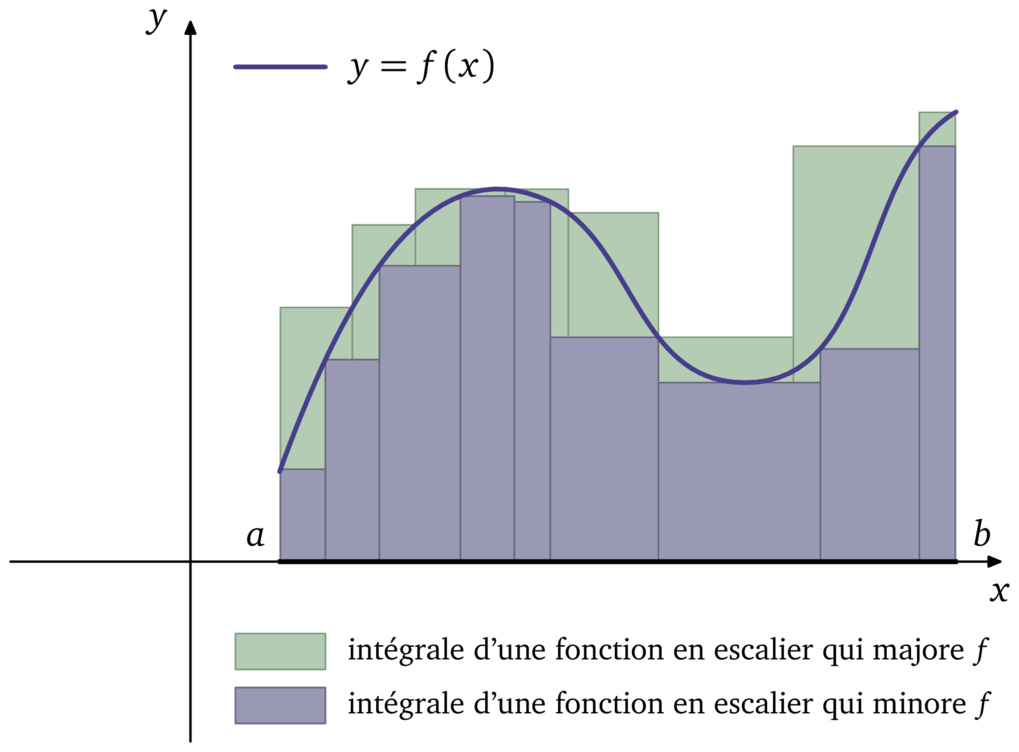
\includegraphics[scale=0.75]{images/002.png} \end{center}

\subsubsection{Remarques}
On peut choisir une subdivision de $[a;b]$ telle que l'aire de $\mathcal{C}_{h-g}$ soit aussi petite que l'on veut.\\

L'intégrale $\displaystyle\int_{a}^{b}(h-g)(x)dx$ est bien définie car h-g est une fonction en escalier (il suffit de prendre comme subdivision $\sigma_h\cup \sigma_g=\sigma_{h-g}$).

\subsubsection{Propriété}
Cette définition implique que toute fonction Riemann-intégrable est bornée.

\subsection{Théorème-Définition}
Soit $f : [a;b] \rightarrow \R$, une fonction définie sur un segment $[a;b]$, on nomme $\xi_-(f)$ l'ensemble des fonctions en escalier sur $[a;b]$ qui minorent $f$ et $\xi_+(f)$ l'ensemble des fonctions en escaliers sur $[a;b]$ qui majorent f.\\

On pose alors $I_-(f)=\underset{g\in\xi_-(f)}{\sup} \displaystyle\int_{a}^{b} g(x)dx$ et $I_+(f)=\underset{h\in\xi_+(f)}{\inf} \displaystyle\int_{a}^{b} h(x)dx$.\\

f est Riemann intégrable sur $[a;b]$ si et seulement si $I_-(f)=I_+(f)$,\\
on a alors $\displaystyle\int_{a}^{b}f(x)dx=I_-(f)=I_+(f)$.

\section{Opérations sur les fonctions Riemann-intégrables}
\subsection{Somme et multiplication par un réel}
Soit $f_1$ et $f_2$ deux fonctions R-intégrables sur un segment $[a;b]$, alors $\lambda f_1+\mu f_2$ est R-intégrable sur $[a;b]$ pour tout $\lambda,\mu\in\R$ et $\displaystyle\int_a^b(\lambda f_1+\mu f_2)(x)dx=\lambda\int_{a}^{b}f_1(x)dx+\mu\int_{a}^{b}f_2(x)dx$.

\subsubsection{Preuve}
On le montre pour des fonctions en escalier $g$ et $h$ : soient $g$ et $h$ deux fonctions en escalier sur $[a;b]$, $(s_i)_{1\leq i\leq n}$ une subdivision de $g$ et de $h$, et $g_i$ et $h_i$ les valeurs de $g$ et $h$ entre $s_i$ et $s_{i+1}$, alors
$$\begin{array}{rcl}\displaystyle\lambda\int_{a}^{b}g(x)dx+\mu\int_{a}^{b}h(x)dx&=&\displaystyle\lambda\sum_{i=0}^{n-1}(s_{i+1}-s_i)g_{i}+\mu\sum_{i=0}^{n-1}(s_{i+1}-s_i)h_{i}=\sum_{i=0}^{n-1}(s_{i+1}-s_i)(\lambda g_{i}+\mu h_{i})\\
&=&\displaystyle\int_{a}^{b}(\lambda g(x)+\mu h(x))dx\end{array}$$\\

Pour $i\in\{1;2\}$, $f_i$ est R-intégrable donc il existe des fonctions $g_i$ et $h_i$ en escalier sur $[a;b]$ telles que $\forall x\in [a;b]$, $g_i(x)\leq f_i(x)\leq h_i(x)$ et $\forall \epsilon>0$, $\displaystyle\int_{a}^{b} (h_i(x)-g_i(x))dx\leq \epsilon$.\\

Si $\lambda>0$, on pose $m_1(x)=\lambda g_1(x)\leq \lambda f_1(x)\leq\lambda h(x)=M_1(x)$ et\\
si $\lambda<0$, on pose $m_1(x)=\lambda h_1(x)\leq \lambda f_1(x)\leq\lambda g_1(x)=M_1(x)$.

Si $\mu>0$, on pose $m_2(x)=\mu g_2(x)\leq \mu f_2(x)\leq\mu h_2(x)=M_2(x)$ et\\
si $\mu<0$, on pose $m_2(x)=\mu h_2(x)\leq \mu f_2(x)\leq\mu g_2(x)=M_2(x)$.\\

$\forall i\in \{1;2\}$, on a donc les fonctions $m_i$ et $M_i$ définies ci-dessus ;\\
$\forall \lambda, \mu\in \R$ (les cas où $\lambda$ ou $\mu$ sont nuls sont triviaux), on a $m_1+m_2\leq \lambda f_1+\mu f_2\leq M_1+M_2$ et $$\displaystyle|\lambda|\int_a^b(h_1-g_1)(x)dx+|\mu|\int_a^b(h_2-g_1)(x)dx<(|\lambda|+|\mu|)\epsilon $$
$$\Leftrightarrow\int_{a}^{b}((M_1+M_2)-(m_1+m_2))(x)dx<(|\lambda|+|\mu|)\epsilon$$
Donc $\lambda f_1+\mu f_2$ est R-intégrable sur $[a;b]$ et $\displaystyle\int_a^b(\lambda f_1+\mu f_2)(x)dx=\lambda\int_{a}^{b}f_1(x)dx+\mu\int_{a}^{b}f_2(x)dx$.

\subsection{Produit}
Soient $f_1$ et $f_2$ deux fonctions R-intégrables sur un segment $[a;b]$, alors la fonction $f_1f_2$ est R-intégrable sur $[a;b]$.

\subsubsection{Preuve}
Soient $f_1$ et $f_2$ deux fonctions R-intégrables (donc bornées), il existe donc des fonctions en escalier $h_i$ et $g_i$ et des nombres $m_i$ et $M_i$ tels que $0\leq g_i\leq f_i(x)-m_i\leq h_i\leq M_i$ et $\forall \epsilon>0$, $0\leq \displaystyle\int_a^b(h_i-g_i)(x)dx\leq \epsilon_i$. De plus, le produit de fonctions en escalier est une fonction en escalier.

$\displaystyle\int_a^b(h_1h_2-g_1g_2)(x)dx=\int_{a}^{b}\left[\frac{1}{2}(h_1-g_1)(h_2+g_2)+(h_2-g_2)(h_1+g_1)\right](x)dx\leq M_2\epsilon_1+M_1\epsilon_2$\\

On a aussi $0\leq g_1g_2\leq (f_1-m_1)(f_2-m_2)\leq h_1h_2$ car $g_i\geq 0$, donc la fonction\\
$F=(f_1-m_1)(f_2-m_2)=f_1f_2-m_1f_2-f_1m_2+m_1m_2$ est R-intégrable et\\
enfin $F+m_1f_2+f_1m_2-m_1m_2=f_1f_2$ est R-intégrable.\\

\newpage

\section{Propriétés des fonctions Riemann-intégrables}
\subsection{Positivité de l'intégrale}
Soit f une fonction R-intégrable sur un intervalle [a;b], si $\forall x\in [a;b]$, $f(x)\geq 0$ alors $$\int_{a}^{b}f(x)dx\geq0$$
La réciproque est fausse.

\subsubsection{Preuve}
La fonction nulle sur $[a;b]$ appartient à $\xi_-(f)$ donc $I_-(f)=\underset{g\in \xi_-(f)}{\sup}\displaystyle\int_{a}^{b}f(x)dx= \int_{a}^{b}f(x)dx$\\
(car $f$ est Riemann-intégrable) sera positive.\\

Soit $f$ la fonction définie sur $[0,2]$ par $f(x)=\left\{\begin{array}{lll}
-1\text{ si }x\in [0;1[ \\
2\text{ sinon }
\end{array} \right.$ dont l'intégrale vaut\\
$\displaystyle\int_0^2 f(x)dx=-1+2=1>0$ mais f n'est pas toujours positive, donc la réciproque est fausse.

\subsection{Passage à l'inégalité}
Soit $f$ et $g$ deux fonctions Riemann-intégrables sur un intervalle $[a;b]$,\\
si $\forall x\in [a;b]$, $f(x)\leq g(x)$ alors $\displaystyle\int_{a}^{b} f(x)dx\leq \int_{a}^{b}g(x)dx$.

\subsubsection{Preuve}
On considère la fonction Riemann-intégrable $g-f\geq 0$ et on applique la propriété précédente.

\subsection{Relation de Chasles}
Soit $f$ une fonction Riemann-intégrable sur un intervalle $[a;b]$, $\forall c\in [a;b]$ on a $$\displaystyle\int_{a}^{c} f(x)dx+\int_{c}^{b}f(x)dx=\int_{a}^{b}f(x)dx$$

\subsubsection{Preuve}
Soit $f_1$ la fonction définie par $f_1(x)=f(x)$ sur $[a;c]$ et $f_1(x)=0$ sinon.

Soit $f_2$ la fonction définie par $f_2(x)=f(x)$ sur $[c;b]$ et $f_2(x)=0$ sinon.\\

Alors $f_1$ et $f_2$ sont R-intégrables sur $[a;b]$, $(f_1+f_2)(x)=f(x)$ sur $[a;b]\backslash\{c\}$,\\
or l'intégrale ne dépend pas de la valeur d'un seul point donc :
$$\displaystyle\int_{a}^{b}f(x)dx=\int_a^b (f_1+f_2)(x)dx=\int_{a}^{b}f_1(x)dx+\int_a^bf_2(x)dx=\int_{a}^{c}f(x)dx+\int_{c}^{b}f(x)dx$$

\newpage

\subsection{Valeur absolue, minimum et maximum}
Soit $f$ et $g$ deux fonctions Riemann-intégrable sur un intervalle $[a;b]$, alors $|f|$, $\max(f,g)$ et $\min(f,g)$ sont Riemann-intégrable et $\left|\displaystyle\int_{a}^{b}f(x)dx\right|\leq \displaystyle\int_{a}^{b}|f(x)|dx$.

\subsubsection{Preuve}
On a $-|f|\leq f\leq |f|$, alors $-\displaystyle\int_{a}^{b}|f(x)|dx\leq \int_{a}^{b}f(x)dx\leq \int_{a}^{b}|f(x)|dx$ et donc $$\left|\int_{a}^{b}f(x)dx\right|\leq \int_{a}^{b}|f(x)|dx$$\\

On a $\max(f,g)=\frac{f+g+|g-f|}{2}$ et $\min(f,g)=\frac{f+g-|g-f|}{2}$ donc les fonctions $\min$ et $\max$ sont aussi Riemann-intégrables sur $[a;b]$.

\subsection{Moyenne}
On appelle moyenne d'une fonction $f$ R-intégrable sur $[a;b]$ le nombre $$\mu=\frac{1}{b-a}\displaystyle\int_{a}^{b}f(x)dx$$

\subsection{Inégalité de la moyenne}
Soient $f$ une fonction R-intégrable sur un ensemble $[a;b]$, $m=\inf(f)$ et $M=\sup(f)$ alors $$m(b-a)\leq \displaystyle\int_{a}^{b} f(x)dx\leq M(b-a)$$

\subsubsection{Preuve}
On a $m\leq f(x)\leq M$, donc avec un passage à l'inégalité on obtient $$\displaystyle\int_{a}^{b}mdx\leq\int_{a}^{b}f(x)dx\leq\int_{a}^{b}Mdx\text{ donc }(b-a)m\leq\int_{a}^{b}f(x)dx\leq (b-a)M$$

\subsection{Formule de la moyenne}
Soit $f$ une fonction R-intégrable continue sur un intervalle $[a;b]$, $m=\inf(f)$ et $M=\sup(f)$ $$\exists c\in [a;b]\text{ }|\text{ }f(c)=\mu=\frac{1}{b-a}\displaystyle\int_{a}^{b}f(x)dx$$

\subsubsection{Preuve}
D'après l'inégalité de la moyenne, $\forall x\in [a;b]$, $m\leq \frac{1}{b-a}\displaystyle\int_a^bf(x)=\mu\leq M$ : $\mu \in [m;M]$ et\\
f est continue donc d'après le théorème des valeurs intermédiaires $\exists c\in [a;b]$ $|$ $f(c)=\mu$.

\newpage

\section{Continuité}
\subsection{Continuité uniforme}
\subsubsection{Définition}
Soit $f : I\rightarrow \R$ définie sur un intervalle, $f$ est uniformément continue sur $I$ si et seulement si $\forall \epsilon>0$, $\exists \eta>0$, $\forall (x,y)\in I^2$, $|x-y|<\eta \Rightarrow |f(x)-f(y)|<\epsilon$.

\subsubsection{Remarque}
La continuité uniforme est une notion plus forte que la continuité simple. Intuitivement, une fonction continue mais non uniformément continue signifie qu'on peut prendre des points arbitrairement proches tels que leurs images ne soient pas arbitrairement proches.

\subsubsection{Théorème de Heine}
Si $f$ est continue sur un segment alors $f$ est uniformément continue sur ce segment.

\subsection{Théorème}
Toute fonction continue sur un segment est Riemann-intégrable.

\subsubsection{Preuve}
$f$ continue sur $[a;b]$ implique $f$ uniformément continue sur [a;b] d'après le théorème de Heine.\\

Alors soit $\epsilon>0$, on a $\eta>0$ donné par l'uniforme continuité de $f$ sur $[a;b]$.\\
Soit $\sigma =(s_i)_{i\in \llbracket 0;n \rrbracket}$ une subdivision de $[a;b]$ de pas $(s_{i+1}-s_i) < \eta$.\\

Ainsi $\forall i\in \llbracket 0;n-1\rrbracket$, $\forall (x;y) \in [s_i,s_{i+1}]^2$ on a $|x-y|\leq |s_{i+1}-s_i|<\eta$ et donc $|f(x)-f(y)|<\epsilon$.\\\\\\
On pose $f_{\sigma}^+ : \begin{array}{rcl} [a;b] &\rightarrow& \R \\ x&\mapsto& \underset{[s_i;s_{i+1}]} {\sup}f \end{array}$ si $x\in [s_i,s_{i+1}]$
et $f_{\sigma}^- : \begin{array}{rcl} [a;b] &\rightarrow& \R \\ x&\mapsto& \underset{[s_i;s_{i+1}]} {\inf}f \end{array}$ si $x\in [s_i,s_{i+1}]$.\\\\

Par construction $f_{\sigma}^+\in \xi_+(f)$ et $f_{\sigma}^-\in \xi_-(f)$.\\

On a $\displaystyle \int_a^b(f_{\sigma}^+-f_{\sigma}^-)(x)dx=\int_{a}^{b}f_{\sigma}^+(x)dx-\int_a^bf_{\sigma}^-(x)dx
=\sum\limits_{i=0}^{n-1}f(b_i)(s_{i+1}-s_i)-\sum\limits_{i=0}^{n-1}f(a_i)(s_{i+1}-s_i)$\\
avec $f(b_i)=\underset{[s_i;s_{i+1}]}{\sup}f$ donc $b_i$ est un antécédent par $f$ de ce $\sup$ \\\\
et $f(a_i)=\underset{[s_i;s_{i+1}]}{\inf}f$ donc $a_i$ est un antécédent par $f$ de cet $\inf$.\\\\

$\displaystyle\int_a^b (f_{\sigma}^+-f_{\sigma}^-)(x)dx=\sum\limits_{i=0}^{n-1}(f(b_i)-f(a_i))(s_{i+1}-s_i)<\sum\limits_{i=0}^{n-1}\epsilon (s_{i+1}-s_i)=\epsilon \sum\limits_{i=0}^{n-1}(s_{i+1}-s_i)=\epsilon(b-a)$\\

car $b_i$ et $a_i \in [s_i;s_{i+1}]$ et $f(b_i)\geq f(a_i)$ donc d'après la continuité uniforme on a $f(b_i)-f(a_i)<\epsilon$.\\\\

Alors $\displaystyle\int_a^b (f_{\sigma}^+-f_{\sigma}^-)(x)dx<\epsilon(b-a)$ et on peut choisir $\sigma$ tel que $\displaystyle\int_a^bf_{\sigma}^+(x)dx$ soit aussi proche que l'on veut de $\displaystyle\int_a^bf_{\sigma}^-(x)dx$.\\

Finalement $f$ est Riemann-intégrable sur [a;b].

\subsubsection{Remarque}
Toute fonction continue par morceaux sur $[a;b]$ (c'est-à-dire continue sauf en un nombre fini de points) est Riemann-intégrable sur $[a;b]$.

\subsubsection{Interprétation géométrique}
Si $f$ est positive sur $[a;b]$, $\displaystyle\int_a^bf(x)dx$ est l'aire du plan défini par les points $(x;y)$ tels que $a\leq x \leq b$ et $0\leq y \leq f(x)$.

\section{Somme de Riemann}
\subsection{Définition}
La somme de Riemann de $f$ relative à une subdivision $\sigma=(s_i)_{i\in\llbracket 0,n \rrbracket}$ de $[a;b]$\\
et à l'ensemble des points $(\theta_i)_{i\in \llbracket0,n-1\rrbracket}$ tels que $\theta_i\in [s_i,s_{i+1}]$ est $\displaystyle\sum\limits_{i=0}^{n-1}f(\theta_1)(s_{i+1}-s_i)$.\\

\begin{center} \begin{tikzpicture}
\draw [domain=0:2*pi, samples=100] plot (\x,{-1.5*cos(\x r)+2}) ;
\draw[->] (-1,-0.5) -- (7,-0.5);
\draw[->] (-0.5,-1) -- (-0.5,4.5);

\node[scale=0.7] at (7.1,-0.5) {$x$};
\node[scale=0.7] at (-0.5,4.7) {$y$};

\draw[densely dashed, thin] (0,-0.5) -- (0,0.5);
\draw[densely dashed, thin] (2,-0.5) -- (2,2.6);
\draw[densely dashed, thin] (4,-0.5) -- (4,2.95);
\draw[densely dashed, thin] (6.28,-0.5) -- (6.28,0.5);

\draw[densely dashed, very thick] (1.5,-0.5) -- (1.5,1.9);
\draw[densely dashed, very thick] (2.5,-0.5) -- (2.5,3.21);
\draw[densely dashed, very thick] (5,-0.5) -- (5,1.61);

\draw[very thick] (0,1.9) -- (2,1.9);
\draw[very thick] (2,3.21) -- (4,3.21);
\draw[very thick] (4,1.61) -- (6.28,1.61);

\node[scale=0.7] at (0.05,-0.7) {$a=S_0$};
\node[scale=0.7] at (2,-0.7) {$S_1$};
\node[scale=0.7] at (4,-0.7) {$S_2$};
\node[scale=0.7] at (6.2,-0.7) {$S_3=b$};

\node[scale=0.7] at (1.5,-0.7) {$\theta_0$};
\node[scale=0.7] at (2.5,-0.7) {$\theta_1$};
\node[scale=0.7] at (5,-0.7) {$\theta_2$};
\end{tikzpicture} \end{center}

\subsection{Théorème}
Si $f$ est Riemann-intégrable sur $[a;b]$, alors les sommes de Riemann de $f$ ont toutes pour limite $\displaystyle\int_a^b f(x)dx$ quand le pas de la subdivision tend vers 0.

\subsubsection{Remarque}
En prenant $\sigma=(s_i)_{i\in\llbracket0,n\rrbracket}$ tel que $\forall i\in \llbracket 0,n \rrbracket$, $s_i=a+\frac{b-a}{n}i$\\
et en prenant $\forall i\in \llbracket 0, n-1 \rrbracket$, $\theta_i=a+\frac{b-a}{n}i$, on obtient la somme de Riemann suivante
$$\sum\limits_{i=0}^{n-1}\frac{b-a}{n}f(a+\frac{b-a}{n}i)$$

Et ainsi si $f$ est Riemann-intégrable sur $[a;b]$ alors 
$$\int_a^bf(x)dx=\lim\limits_{n\rightarrow +\infty}\left( \sum\limits_{i=0}^{n-1} \frac{b-a}{n}f(a+i\frac{b-a}{n}) \right)$$

\newpage

\section{Primitives de fonctions continues}
\subsection{Définition}
Soit $f : D_{f}\subseteq \R \rightarrow \R$ continue sur $D_f$, on appelle primitive de $f$ sur $D_f$\\
toute fonction $F$ dérivable sur $I$ dont la dérivée est $f$.

\subsection{Propriété}
Soit $F$ une primitive de $f$ sur $D$, l'ensemble des primitives de $f$ sur $D$ est l'ensemble des fonctions $F+C$ avec $C$ une fonction constante sur chaque intervalle de $D$ (si $D$ est une réunion d'intervalles).

\subsection{Théorème fondamental de l'analyse}
Soient $f$ une fonction continue sur un intervalle $I$ et $a\in I$.\\

La fonction $F_a:x\mapsto \displaystyle\int_a^xf(t)dt$ est l'unique primitive qui s'annule en $a$ et\\
pour toute primitive $F$ de $f$ sur $I$, on a $F_a(x)=F(x)-F(a)$.

\subsubsection{Démonstration}
Soit $x_0\in I$, on veut montrer que $F_a$ est dérivable en $x_0$.\\\\
$\forall h\in \R^*$ tel que $x_0+h\in I$, on a $\frac{F_a(x_0+h)-F_a(x_0)}{h}=\frac{1}{h}\left(\displaystyle\int_{a}^{x_0+h}f(t)dt-\displaystyle\int_{a}^{x_0}f(t)dt\right)=\frac{1}{h}\displaystyle\int_{x_0}^{x_0+h}f(t)dt$.\\\\

D'après la formule de la moyenne $\exists c_h\in [x_0;x_0+h]$ (ou $[x_0+h;x_0]$ si $h<0$)\\
tel que $f(c_h)=\frac{1}{h}\displaystyle\int_{x_0}^{x_0+h}f(t)dt$ or $\lim\limits_{h\rightarrow 0}c_h=x_0$.\\\\

Donc on a $\lim\limits_{h\rightarrow 0} \frac{F_a(x_0+h)-F_a(x_0)}{h}=\lim\limits_{h\rightarrow 0}\frac{1}{h}\displaystyle\int_{x_0}^{x_0+h}f(t)dt=\lim\limits_{h\rightarrow 0}f(c_h)=f(x_0)$.\\\\

Ainsi la limite du taux d'accroissement existe donc $F_a$ est dérivable en $x_0$ et $F_a'(x_0)=f(x_0)$
(de plus $f$ est continue donc $F_a$ est de classe $\mathcal{C}^1$ sur $I$) donc $F_a$ est bien une primitive de $f$ sur $I$.\\\\

$F_a$ s'annule en $a$ car $\displaystyle\int_{a}^{a}f(t)dt=0$. De plus toute primitive $F$ de $f$ sur $I$ diffère de $F_a$ d'une constante : $\forall x\in I$, $F(x)=F_a(x)+c$.\\\\

On a $F(a)=F_a(a)+c=c$ d'où $F_a(x)$ est l'unique primitive de $f$ qui s'annule en $a$.

\subsubsection{Remarque}
Si l'on connaît une primitive $F$ de $f$, on peut calculer $\displaystyle\int_a^b f(t)dt=[F(x)]_a^b=F(b)-F(a)$.\\

En effet, $\displaystyle\int_a^bf(t)dt=F_a(b)=F(b)-F(a)$ avec $F_a$ la primitive qui s'annule en $a$ et\\
$F$ une primitive quelconque.

\newpage

\section{Calcul des primitives}
\subsection{Primitives usuelles}
\subsubsection{Fonctions hyperboliques}
On appelle sinus hyperbolique et cosinus hyperboliques respectivement la partie impaire et la partie paire de $e^x$ : $\sinh(x)=\frac{e^x-e^{-x}}{2}$ et $\cosh(x)=\frac{e^x+e^{-x}}{2}$.\\

De plus, $(\sinh)'=\cosh$ et $(\cosh)'=\sinh$.

\subsubsection{Primitives communes}

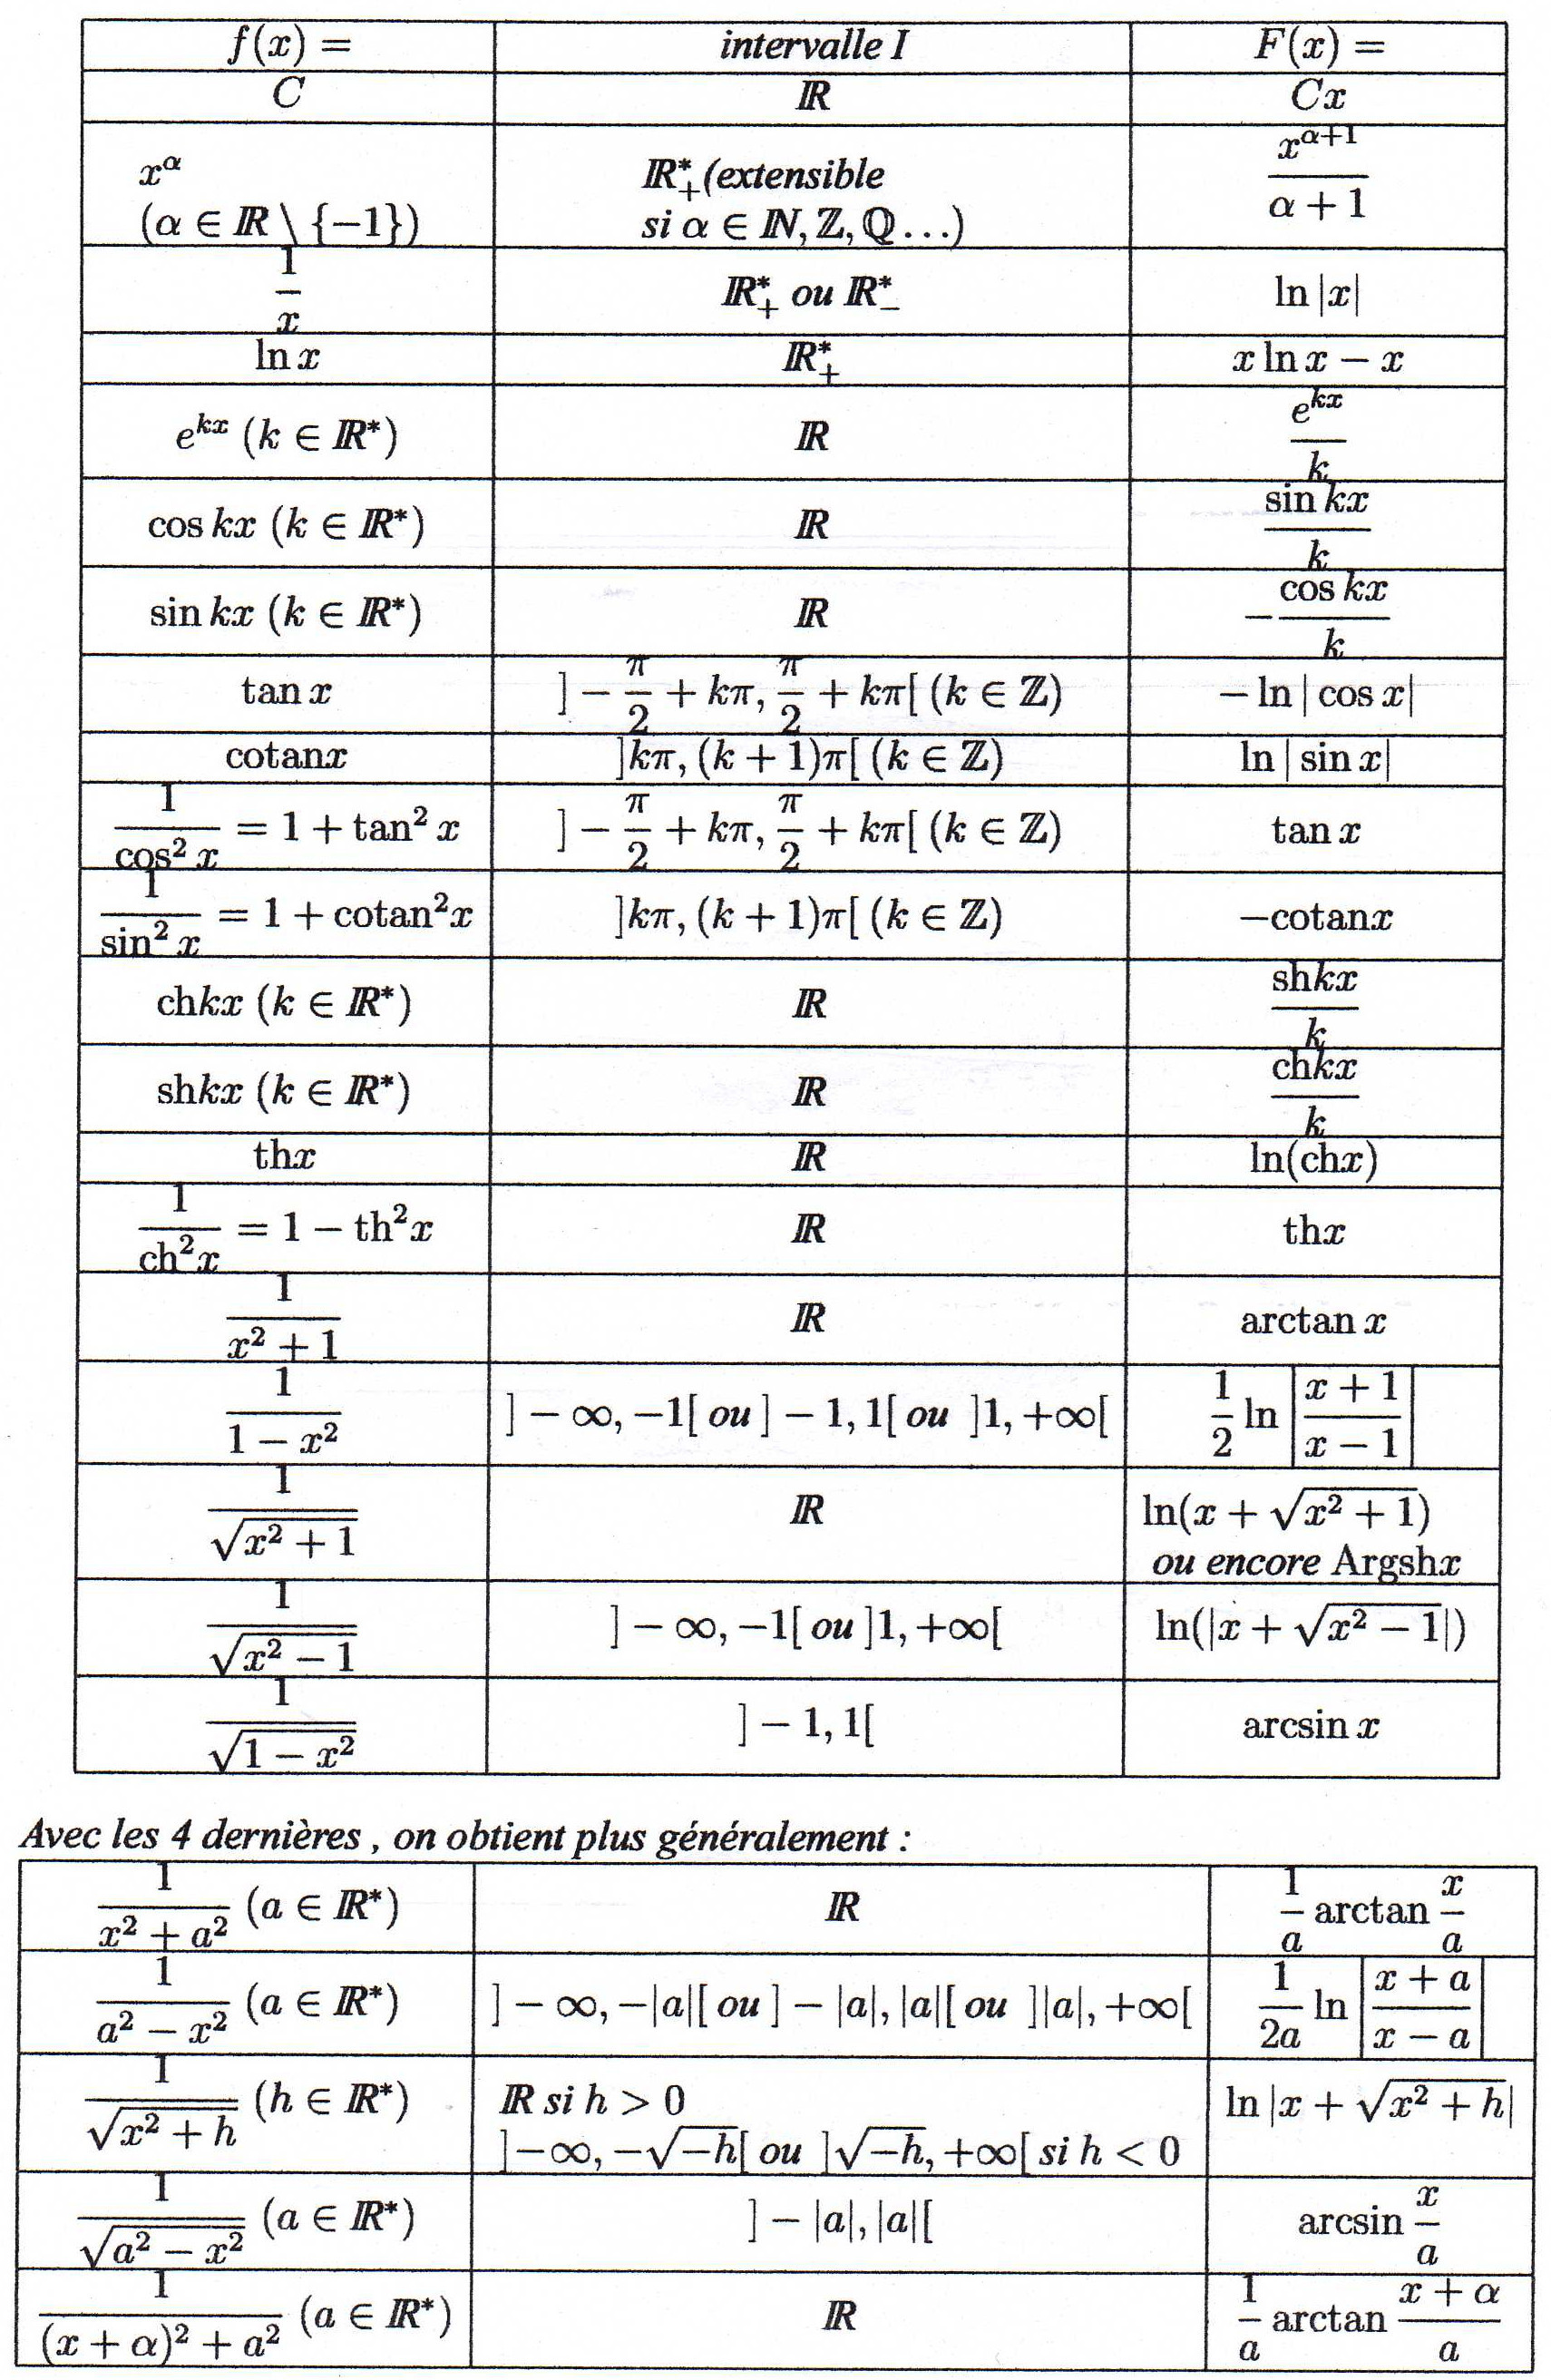
\includegraphics[scale=0.2,angle=0.2]{images/003.jpg}

\newpage

\subsection{Théorème}
Si $f:[a;b]\rightarrow \R$ est continue positive, alors $\displaystyle\int_{a}^{b} f(t)dt=0\Leftrightarrow f=0$ sur $[a;b]$.

\subsubsection{Preuve}
$f=0 \Rightarrow \displaystyle\int_{a}^{b}f(t)dt=0$.\\\\

\emph{Réciproquement :}\\\\
On a $f\geq 0$ sur $[a;b]$, notamment $f\geq 0$ sur $[a;x]$ avec $x\in [a;b]$ et idem sur $[x;b]$.\\

Donc $\displaystyle\int_{a}^{x}f(t)dt\geq 0$ et $\displaystyle\int_{x}^{b}f(t)dt\geq 0$ or $\displaystyle\int_{a}^{x}f(t)dt+\int_{x}^{b}f(t)dt=\int_{a}^{b}f(t)dt=0$ par hypothèse,\\
donc $\displaystyle\int_{a}^{x}f(t)dt=\int_{x}^{b}f(t)dt=0$ et $\displaystyle\left(\int_{a}^{x}f(t)dt\right)'=f(x)=0$.

\subsection{Intégration par partie}
Soit $u$ et $v$ deux fonctions de classe $\mathcal{C}^1$ sur $[a;b]$, on a $$\int_a^bu'(x)v(x)dx=[u(x)(v(x))]_a^b-\int_{a}^{b}u(x)v'(x)dx.$$

\subsubsection{Preuve}
$u$, $v$, $u'$ et $v'$ sont continues sur $[a;b]$
donc $u'v$ et $v'u$ sont primitivables sur $[a;b]$
et comme $(uv)'=u'v+uv'$, $uv$ est une primitive de $u'v+uv'$ sur $[a;b]$
donc $\displaystyle\int_a^b(u'v+uv')(x)dx=[(uv)(x)]_a^b$.

\subsection{Changement de variable}
Soit $f$ une fonction continue sur un intervalle $I$ et $\phi$ une fonction de classe $\mathcal{C}^1$ sur [a;b] à valeur dans $[a;b]$, alors on a
$$\int_{a}^{b}(f\circ\phi)\phi'(x)dx=\int_{\phi(a)}^{\phi(b)}f(t)dt.$$

\subsubsection{Preuve}
On pose $F$ une primitive de $f$ sur $I$.
$(F\circ \phi)'=\phi'\times (f\circ\phi)$ est continue sur $[a;b]$. Alors
$$\displaystyle\int_{a}^{b}(f\circ \phi(x))\phi'(x)=F\circ\phi(b)-F\circ \phi(a)=\int_{\phi(a)}^{\phi(b)}f(t)dt.$$

\subsubsection{Remarque}
Il ne faut pas oublier de vérifier que $\phi$ est de classe $\mathcal{C}^1$ sur $[a;b]$ (notamment $\phi'$ est continue sur $[a;b]$).

\newpage

\section{Primitives de fonctions rationnelles}
\subsection{Principe}
On cherche à calculer la primitive d'une fonction $f$ de la forme $f=\frac{P}{Q}$ où $P,Q\in\R[X]$.\\

On pose $\frac{P}{Q}=T+\frac{R}{Q}$ où $T$ est le quotient de la division euclidienne de $P$ par $Q$ et $R$ le reste.\\
Ainsi on a $\deg(R)<\deg(Q)$ et $\deg(T)=\deg(P)-\deg(Q)$.

\subsection{Théorème de la décomposition en éléments simples}
Soit $\frac{R}{Q}$ une fraction rationnelle avec $R,Q\in \R[X]^{2}$, $R$ premier avec $Q=(X-\alpha_{1})^{k_{1}}...(X-\alpha_{r})^{k_{r}}$.\\

Alors il existe une et une seule écriture de $\frac{R}{Q}$ telle que :
$$\frac{R}{Q}=\sum\limits_{i=1}^p\sum\limits_{j=1}^{k_i}
\frac{\rho_{i,j}}{(X-r_i)^j}+\sum\limits_{i=1}^{q}\sum\limits_{j=1}^{n_i} \frac{\gamma_{i,j}X+\mu_{i,j}}{(X^2+a_iX+b_i)^j}$$
où $\rho_{i,j}$, $\mu_{i,j}$ et $\gamma_{i,j}$ sont des constantes potentiellement toutes différentes dépendant de $i$ et de $j$, et $\displaystyle\frac{\rho_{i,j}}{(X-r_i)^{j}}$ et $\displaystyle\frac{\gamma_{i,j}X+\mu_{i,j}}{(X^2+a_iX+b_i)^j}$ sont des éléments simples sur $\R[X]$.\\

\subsection{Intégration}
\subsubsection{Élément simple de $1^{\text{ère}}$ espèce}
Les éléments simples de première espèce sont les éléments de type $\displaystyle\frac{\rho_{i,j}}{(X-r_i)^j}$ :

$$\displaystyle\int\frac{\rho_{i,j}dX}{(X-a)^n}=\left\{ \begin{array}{ccl}
\rho_{i,j}\ln(|X-a|) &\text{ si }n=1 & \\
\displaystyle\frac{\rho_{i,j}}{(1-n)(X-a)^{n-1}} &\text{ si }n>1 &
\end{array}\right.$$


\subsubsection{Élément simple de $2^{\text{nd}}$ espèce}
Les éléments simples de seconde espèce sont les éléments du type $\displaystyle\frac{\gamma_{i,j}X+\mu_{i,j}}{X^2+a_iX+b_i}$
(où $a_i{}^2<4b_i$) :\\

On écrit $X^2+a_iX+b_i$ sous la forme canonique $(X-\alpha)^2+\beta^2$ avec $\alpha=-\frac{a_i}{2}$ et $\beta=\frac{\sqrt{4b_i-a_i{}^2}}{2}$, et on pose $t=\frac{X-\alpha}{\beta}$ donc $X=\beta t+\alpha$, $dX=\beta dt$ et $X^2+a_iX+b_i=\beta^2(t^2+1)$.\\

$$\displaystyle\int\frac{\gamma_{i,j}X+\mu_{i,j}}{(X^2+a_iX+b_i)^n}dX=\int\frac{\gamma_{i,j}(\beta t+\alpha)+\mu_{i,j}}{\beta^{2n}(t^2+1)^n}dt=\frac{\gamma_{i,j}}{\beta^{2n-1}}\int\frac{tdt}{(t^2+1)^n}+ \frac{\gamma_{i,j}\alpha+\mu_{i,j}}{\beta^{2n}}\int\frac{dt}{(t^2+1)^n}$$\\\\

\textbf{Première intégration}\\
$$\displaystyle\int \frac{tdt}{(t^2+1)^n}=\left\{\begin{array}{ccl}\displaystyle\frac{1}{2}\ln(1+X^2)&\text{ si }n=1 &\\
\displaystyle\frac{1}{(2-2n)(1+X^2)^{n-1}}&\text{ si }n>1 &\end{array}\right.$$\\

\newpage

\textbf{Seconde intégration}
$$\int\frac{dt}{(t^2+1)^n}=\left\{\begin{array}{ccl}
\arctan(X)&\text{ si }n=1& \\
\displaystyle\frac{X}{(2n-2)(1+X^2)^{n-1}}+\frac{2n-3}{2n-2}\int\frac{dt}{(t^2+1)^{n-1}}&\text{ si }n>1&
\end{array}\right.$$\\

\textbf{\phantom{aaaa}Preuve}\\
Si $n>1$, on intègre $\displaystyle\int\frac{dt}{(1+t^2)^{n-1}}$ par partie avec $\displaystyle u(t)=\frac{1}{(1+t^2)^{n-1}}$ et $\displaystyle u'(t)=\frac{2(1-n)t}{(1+t^2)^n}$:

$$\displaystyle\int\frac{dt}{(1+t^2)^{n-1}} =\frac{X}{(1+X^2)^{n-1}}-\int\frac{2(1-n)t^2dt}{(1+t^2)^n} =\frac{X}{(1+X^2)^{n-1}}- 2(1-n) \int\frac{t^2dt}{(1+t^2)^n}$$
Or $\displaystyle\frac{t^2}{(1+t^2)^n} =\frac{1+t^2-1}{(1+t^2)^n} =\frac{1}{(1+t^2)^{n-1}}-\frac{1}{(1+t^2)^n}$\\\\

d'où $\displaystyle\int\frac{dt}{(1+t^2)^{n-1}} =\frac{X}{(1+X^2)^{n-1}}+\int\frac{2n-2}{(1+t^2)^{n-1}}dt -\int\frac{2n-2}{(1+t^2)^n}dt$\\\\

$\Leftrightarrow\displaystyle(2n-2)\int\frac{dt}{(1+t^2)^n} =\frac{X}{(1+X^2)^{n-1}}+ (2n-3)\int\frac{dt}{(1+t^2)^{n-1}}$\\\\

Enfin $\displaystyle\int\frac{dt}{(1+t^2)^n} =\frac{X}{(2n-2)(1+X^2)^{n-1}}+ \frac{2n-3}{2n-2}\int\frac{dt}{(1+t^2)^{n-1}}$

\subsection{Intégration de fonctions rationnelles en $\sin(t)$ et $\cos(t)$}
\subsubsection{Principe}
On pose $f(t)$ une expression rationnelle en $\sin(t)$ et $\cos(t)$ c'est-à-dire $f(t)=\frac{P(\cos(t),\sin(t))}{Q(\cos(t),\sin(t))}$\\
avec P et S des polynômes bivariés à coefficients réels.\\

Pour calculer $\displaystyle\int f(t)dt$, on procède à un changement de variable pour se ramener au problème d'intégration de fonction rationnelles réelles.\\

Pour choisir ce changement de variable, on applique la règle de Bioche, 

\subsubsection{Règle de Bioche}
On choisit la fonction $u$ en fonction des conditions ci-dessous :\\
(si deux des trois premières conditions sont vérifiées, la 3e l'est aussi et on prend $u(t)=\cos(2t)$)


\begin{enumerate}
\item Si $f(-t)d(-t)=f(t)dt$, alors $u(t)=\cos(t)$.
\item Si $f(\pi-t)d(\pi-t)=f(t)dt$ alors $u(t)=\sin(t)$.
\item Si $f(\pi+t)d(\pi+t)=f(t)dt$ alors $u(t)=\tan(t)$.
\item Si aucune des relations précédentes n'est vraie alors on posera généralement $u(t)=\tan(\frac{t}{2})$\\

En effet en prenant $u(t)=\tan(\frac{t}{2})$, on se retrouve avec $\tan(x)=\frac{2t}{1-t^2}$, $\sin(x)=\frac{2t}{1+t^2}$ et $\cos(x)=\frac{1-t^2}{1+t^2}$, qui sont des expressions polynomiales.
\end{enumerate}


% ------------------------------------------------------------------------------------------------------ %
% ------------------------------------------------------------------------------------------------------ %



% ------------------------------------------------------------------------------------------------------ %
% ------------------------------------------------------------------------------------------------------ %


\chapter{Équations différentielles linéaires}
\section{Généralités}
\subsection{Définition}
\subsubsection{Forme générale}
La forme générale d'une équation différentielle linéaire est 
$$(E):\text{ } a_ny^{(n)}+\cdots+a_1y'+a_0y=b$$
avec $y$ la fonction recherchée et $(a_i)_{0\leq i\leq n}$ et $b$ des fonctions réelles continues.

\subsubsection{Résolution}
Résoudre une telle équation sur un intervalle particulier $I\subseteq \R$ consiste à déterminer l'ensemble $S_E$ des fonctions $y\in \mathcal{C}^n(I,\R)$ telles que l'égalité $E$ soit vérifiée sur $I$.

\subsubsection{Équation homogène}
La fonction $b$ est appelée le second membre, si $b$ est nulle, l'équation $E$ est dite homogène.\\\\
L'équation différentielle linéaire homogène $(H)$ associée à $(E)$ est $$(H):\text{ }a_ny^{(n)}+\cdots+a_1y'+a_0y=0$$

\subsection{Structure de l'ensemble des solutions d'une équation différentielle linéaire}
Soit $(E)$ une équation différentielle linéaire, si $y_0$ est une solution particulière de $(E)$ alors l'ensemble des solutions sont les fonctions de la forme $y_0+y_h$ où $y_h$ décrit l'ensemble des solutions de l'équation homogène associée à $(E)$.

\subsection{Propriété}
L'ensemble $S_H$ des solutions d'une équation homogène est un sous-espace vectoriel de $\mathcal{C}^1(I,\R)$.

\subsubsection{Démonstration}
$S_H$ possède toujours au moins un élément : la fonction nulle.\\
De plus, toute combinaison linéaire d'éléments de $S_H$ est un élément de $S_H$.

\subsubsection{Remarque}
Ainsi l'ensemble $S_E$ des solutions d'une équation différentielle linéaire est un espace affine de $\mathcal{C}^1(I,\R)$ de direction $S_H$.

\newpage

\subsection{Principe de superposition}
Si $\forall i \in A\subseteq \N$, $y_i$ est solution de l'équation différentielle linéaire $\displaystyle\sum_{k=0}^n a_ky^{(k)}=b_i$,\\
alors $\forall (\lambda_i)\in\R$, $\displaystyle\sum\lambda_iy_i$ est solution de l'équation différentielle linéaire $\displaystyle\sum\limits_{k=0}^na_ky^{(k)}=\sum\lambda_ib_i$.

\subsection{Nomenclature}
\subsubsection{Prolongement}
Soit l'équation différentielle $E$ et soit $y_1 \in \mathcal{C}^1(I_1,\R)$ une solution de $E$ sur $I_1$ et $y_2$ une solution sur $I_2$.\\

On dit que $y_2$ est un prolongement de $y_1$ si $I_1\subseteq I_2$ et $\forall x\in I_1$, $y_1(x)=y_2(x)$.

\subsubsection{Solution maximale}
Une solution est dite maximale si elle n'admet pas de prolongement.

\section{Équation différentielle linéaire d'ordre 1}
\subsection{Définition}
On appelle équation différentielle linéaire homogène du premier ordre toute équation\\
différentielle de la forme $(H) :$ $y'+ay=0$ d'inconnue $y\in \mathcal{C}^1(I\subseteq\R,\R)$ avec\\
$a$ une fonction réelle continue de $\mathcal{C}^1(I,\R)$.

\subsection{Solution de l'équation homogène}
L'ensemble de $(H)$ sur $I$ est $S_H=\left\{ y: \begin{array}{rcl}I&\rightarrow& \R \\ x&\mapsto& \lambda e^{-A}\end{array}\text{, }\lambda\in \R\right\}$
avec $A$ une primitive de $a$.

\subsubsection{Démonstration}
On a $(ye^A)'=y'e^A+aye^A=e^A(y'+ay)$.\\
Soit $y_H$ une solution de $(H)$ alors $y_H'+a_{y_H}=0 \Leftrightarrow (y_He^A)'=0$.\\
Donc $y_H'+ay_H=0 \Leftrightarrow y_He^A=\lambda$, $\lambda\in \R$\\

Enfin $y_H$ est solution de $(H)$ sur $I$ si et seulement si $y_H$ est de la forme $y_H:x\mapsto \lambda e^{-A(x)}$, $\lambda\in \R$.\\

Réciproquement, on vérifie que toute fonction de la forme $\lambda e^{-A}$ avec $\lambda \in \R$ vérifie l'\edlh $(H)$ :\\
$$(\lambda e^{-A})'+a\lambda e^{-A}=-\lambda A'+a\lambda e^{-A}=-\lambda ae^{-A}+a\lambda e^{-A}=0$$

\subsection{Solutions de l'équation avec un second membre}
\subsubsection{Définition}
On appelle \edl du premier ordre toute équation différentielle du type $(E)$ $y'+ay=b$ d'inconnue $y\in \mathcal{C}^1(I,\R)$ avec $a$ et $b$ des fonctions réelles continues.

\subsubsection{Résolution}
Pour résoudre $E$ on résout l'équation homogène $H$ associée à $E$ puis on recherche une solution particulière $y_0$. L'ensemble des solutions de $E$ est l'espace affine $y_0+S_H$ avec $S_H$ l'ensemble des solutions de $(H)$.

\subsubsection{Solution particulière}
Pour trouver une solution particulière, on peut :\begin{itemize}
\item en trouver une évidente
\item utiliser le principe de superposition
\item utiliser la méthode de résolution par variation de la constante\\\end{itemize}

\subsubsection{Solution}
Pour résoudre $E$ on résout l'équation homogène associée $H$ et on remplace, dans l'expression de la solution générale, la constante arbitraire $\lambda$ par une fonction inconnue $\lambda(x)$ dont la détermination fournit une solution générale de $E$.

\subsection{Généralisation}
On s’intéresse au cas où l'\edl est de la forme $Ay'+By=C$ d'inconnue $y\in \mathcal{C}^1(I,\R)$ avec $A$,$B$ et $C$ des fonctions réelles continues.\\

On se ramène, sur tout sous-intervalle $J\subseteq I$ où $A$ ne s'annule pas, à l'équation $y'+ay=b$ en posant $a=\frac{B}{A}$ et $b=\frac{C}{A}$.\\

\subsection{Théorème}
\textit{Résolution du problème de Cauchy}\\

Soit une \edl $E$ et $S_E$ son ensemble de solution dans $\mathcal{C}^1(I,\R)$.\\
Soient $x_0 \in  I\subseteq \R$ et $\alpha \in \R$.\\

Il existe une unique solution $y_0\in S_E$ tel que $y_0(x_0)=\alpha$.\\\\
Pour résoudre ce genre de problème, on résout le système constitué d'une solution générale paramétrée dans $\R$ et de l'équation $y_0(x_0)=\alpha$.

\subsection{Équation différentielle linéaire à variables séparables}
Une \edl du type $y'\times g(y)=h$ d'inconnue $y \in \mathcal{C}^1(I,\R)$ avec $g$ et $h$ des fonctions réelles continues est dite à variables séparables.

\subsubsection{Résolution}
Soit $(E)$ une \edl à variables séparables :
$$(E)\text{: } y'\times g(y)=h$$\\

Soient $G$ et $H$ des primitives respectives de $g$ et $h$,
la solution générale de $E$ est donnée par $$G(y)=H+\lambda\text{, }\lambda\in \R$$

\newpage

\section{Équation différentielle d'ordre 2 à coefficients constants}
\subsection{Définition}
\subsubsection{Équation différentielle linéaire d'ordre 2 à coefficient constant}
On s’intéresse ici aux équations différentielles linéaires du second ordre de la forme $$(E)\text{: } \alpha y''+\beta y'+\gamma y=d$$
d'inconnue $y\in \mathcal{C}^2(I,\R)$ avec $\alpha,\beta,\gamma\in \R^3$ ($\alpha\neq 0$) et $d$ une fonction réelle continue.

\subsubsection{Équation homogène}
L'équation homogène $(H)$ associée à $(E)$ est $$(H)\text{: } \alpha y''+\beta y'+\gamma y=0$$

\subsubsection{Ensemble des solutions}
L'ensemble $S_H$ des solutions de $H$ est un espace vectoriel de dimension 2 de $\R$ ($S_H~\R^2$).

L'ensemble des solutions de $E$ est un espace affine de direction $S_H$.

\subsection{Résolution de l'équation homogène}
\subsubsection{Équation caractéristique}
On appelle équation caractéristique de $(H)$ l'équation du second degré 
$$(H_c)\text{: }\alpha x^2+\beta x+\gamma=0$$
On note $\Delta=\beta^2-4\alpha\gamma$ le discriminant de $(H_c)$.

\subsubsection{Discriminant positif}
Si $\Delta>0$, alors $(H_c)$ a 2 racines réelles $\displaystyle r_1=\frac{-\beta-\sqrt{\Delta}}{2\alpha}$ et $\displaystyle r_2=\frac{-\beta+\sqrt{\Delta}}{2\alpha}$.\\

L'ensemble des solutions de $(H)$ est alors $$S_H=\left\{ \lambda_1e^{r_1x}+\lambda_2e^{r_2x}, (\lambda_1;\lambda_2)\in\R^2 \right\}$$

\subsubsection{Discriminant nul}
Si $\Delta=0$, alors $(H_c)$ a une racine réelle double $\displaystyle r=\frac{-\beta}{2\alpha}$.\\

L'ensemble des solutions de $(H)$ est alors $$S_H=\left\{ e^{rx}(\lambda_1x+\lambda_2) , (\lambda_1;\lambda_2)\in\R^2 \right\}$$

\subsubsection{Discriminant négatif}
Si $\Delta<0$, alors $(H_c)$ admet deux racines complexes conjuguées $r_1$ et $r_2$,\\
on pose $\rho=\Re(r_1)=\Re(r_2)=\frac{-\beta}{2\alpha}$ et $\tau=|\Im(r_1)|=|\Im(r_2)|= |\frac{\sqrt{-\Delta}}{2\alpha}|$.\\

L'ensemble des solutions de $(H)$ est alors
$$S_H=\left\{ e^{\rho x}(\lambda_1\cos(\tau x)+\lambda_2\sin(\tau x)\text{, }(\lambda_1;\lambda_2)\in\R^2 \right\}$$

\subsubsection{Remarque}
On retrouve que $S_H \sim \R^2$.

\newpage

\subsection{Résolution avec second membre}
Soit $(E)$ une équation différentielle du second ordre telle que $(E)\text{: } \alpha y''+\beta y'+\gamma y=d$.

\subsubsection{Principe général}
Les solutions $y$ de $(E)$ sont toutes de la forme :
$$y=y_H+y_P$$
où $y_H$ est la forme générale des solutions de $(H)$ et $y_P$ est une solution particulière de $(E)$.

\subsubsection{Preuve}
Soit $y$ une solution de (E) et $y_P$ une solution particulière.\\
Si on pose $z(x)=y(x)-y_P(x)$ alors :
$$az"(x)+bz'(x)+cz(x)=ay"+by'+cy-ay_P"-by_P'-cy_P=d(x)-d(x)$$
Ainsi $z$ est une solution de $(H)$ c'est à dire, $z=y_H$, et donc $y_E=y_H+y_P$.

\subsubsection{Conclusion}
Sachant que l'on sait résoudre $(H)$, pour résoudre $(E)$ il faut trouver une solution particulière.

\subsubsection{Solution particulière}
\begin{itemize}[label=$\bullet$]
\item $d(x)$ est un polynôme\\
Si $d$ est un polynôme, l'équation $(E)$ admet une solution particulière qui est un polynôme de degré inférieur ou égal à $\deg(d)+2$.\\

\textit{Démonstration :}\\
On se ramène à un calcul algébrique puis on résout un système linéaire "diagonal".\\

\item $d(x)=P(x)e^{mx}$ avec P(x) un polynôme et $m\in \R$\\
Si $d(x)=P(x)e^{mx}$, $(E)$ admet une solution particulière $y_P$ de la forme $y_P(x)=z(x)e^{mx}$ \\
où $z$ est un polynôme de degré inférieur ou égal à $deg(P)+2$.\\

\item $d(x)$ est une somme de produit de polynômes et d'exponentielles\\
On utilise alors le principe de superposition.

\subsubsection{Principe de superposition}
Si $d(x)=d_1(x)+d_2(x)$ :\\
$y_1$ est solution particulière de :
$$ay"+by'+cy=d_1(x)$$
$y_2$ est une solution particulière de :
$$ay"+by'+cy=d_2(x)$$
Alors $y_P$=$y_1+y_2$ est une solution particulière de :
$$ay"+by'+cy=d(x)$$

\subsubsection{Preuve}
On remplace $y$ par $y_P$ et on trouve le résultat attendu.

\end{itemize}







\end{document}